\documentclass[11pt]{article}
\usepackage[a4paper,margin=1in]{geometry}
\usepackage{microtype}
\usepackage{parskip}
\usepackage{amsmath}
\usepackage{amssymb}

\usepackage{graphicx}
\usepackage{subcaption}
\usepackage{booktabs}
\usepackage{array}
\usepackage{tikz}

\usepackage{framed}


\usepackage[colorlinks=true,
            linkcolor=black,
            citecolor=black,
            urlcolor=blue!60!black]{hyperref}

%% SUGGESTION: The repository is named "SPHINCS-Parameters" but this title says "SHRINCS".
%% Decide which name is canonical and use it consistently throughout the document.
%% (If "SHRINCS" is intentional — the hybrid construction's own name — consider a short
%% footnote on first mention to disambiguate it from SPHINCS+/SLH-DSA.)
\title{SHRINCS Parameter Search Methodology}
\date{\today}

\begin{document}

\maketitle

\tableofcontents
\vspace{1em}

\section{Introduction} \label{sec:introduction}

In the case of Bitcoin, hash-based signature schemes are the most compatible among all quantum-resistant signature algorithms.  Still, the smallest stateless hash-based signature proposed by NIST (SLH-DSA-128s) is 7,856 bytes, which is more than 100$\times$ larger than the current Schnorr signature. The question is whether we can have something smaller and more practical without significant deviation from the standard?

SHRINCS proposes a hybrid signature that consists of a stateful and a stateless part, varying the signature size from \emph{324} (stateful) to \emph{X} (stateless) bytes. This document tries to answer the question of what the value of \emph{X} might be while keeping other signature metrics (KeyGen, SigGen, SigVer, etc) practical.

In this document, we show the methodology of searching parameters for SLH-DSA-compatible signatures: how changes in the hypertree structure and other parameters can affect the signature metrics. Unfortunately, as mentioned before, we keep ourselves in very conservative bounds and avoid any changes in signature sub-algorithms to make the signature as compatible as possible with the SLH-DSA standard. 

\textit{Sometimes we will refer to amazing proposals, like hypertree pruning and +C compression techniques, which allow us to achieve even better shrinking results. Although some of them can be considered as partially compatible, we do not rely on them in the evaluation framework. We still think it's useful to present the potential capabilities of such techniques and allow the reader to tweak the parameters based on them.} 
\section{Parameters Description}

\subsection{Initial Parameters}

As mentioned in the introduction, our objective is to find such parameters that will be better than SLH-DSA. 
For the Bitcoin we require no more than 128-bit security. 
If we put the security cap higher this will lead to bigger signature size and costs, which is not preferable.
Another parameter that sets the further foundation for the parameter search is the number of signatures, namely $q_{s}$. 
In SLH-DSA-128s version, the number of signatures is set to be $q_{s} = 2^{64}$. 
While parameters for standardized SLH-DSA are created for general purpose usage, the number of required signatures in Bitcoin is lower.
Setting $q_{s} = 2^{40}$ is enough for our purposes, which will decrease the size and the computational cost.

\subsection{SLH-DSA Parameters}

The basic architecture of SLH-DSA relies on a hyper-tree of extended Merkle signature schemes (XMSS) to authenticate underlying one-time and few-time signature keys. 
We formally parameterize each candidate configuration using the tuple $(h, d, k, a, w)$, where each variable controls a distinct geometric trade-off within the overall structure.

\paragraph{Hyper-Tree Geometry ($h$ and $d$)}
The hyper-tree configuration determines the capacity and layer traversal costs of the signature scheme.
\begin{itemize}
    \item $h$ represents the total height of the multi-layered hyper-tree. 
    This variable dictates the maximum number of few-time signature instances supported at the base layer, yielding a total capacity of $2^h$ unique leaf nodes.
    \item $d$ defines the number of independent tree layers comprising the hyper-tree. 
\end{itemize}
To ensure symmetrical construction across all internal boundaries, our search pipeline strictly mandates that the total height $h$ must be perfectly divisible by the layer count $d$. 
Consequently, each individual XMSS tree layer operates with a uniform height denoted as $h'$:
\begin{equation*}
    h' = \frac{h}{d}
\end{equation*}
Adjusting the ratio between $h$ and $d$ governs the balance between signature size and key generation speed. 
Minimizing layers ($d$) reduces the total number of intermediate public keys and authentication paths included in the signature payload, saving valuable bytes. 
However, this exponentially increases the height $h'$ of each constituent tree layer, requiring significantly more hash operations to compute the root node during key generation.

\paragraph{Few-Time Signature Layer ($k$ and $a$)}
The lowest layer of the hyper-tree authenticates the Forest of Random Subsets (FORS) few-time signature scheme, which directly signs the message digest.
\begin{itemize}
    \item $k$ represents the number of independent, parallel Merkle trees operating within the FORS layer.
    \item $a$ defines the height of each individual FORS tree. This parameter dictates that each constituent tree contains exactly $t = 2^a$ leaves.
\end{itemize}

Increasing $k$ and $a$ strengthens the scheme against multi-target subset forgery attacks, allowing the structure to safely support larger capacities. 
However, expanding these dimensions directly increases the byte footprint of the appended authentication paths.

\paragraph{One-Time Signature Base ($w$)}
Internal tree roots are signed using the Winternitz One-Time Signature Plus (WOTS+) scheme. 
The base parameter $w$ defines the underlying digit representation used to split the message digest during signing. 
Our framework evaluates candidate configurations across standard baseline settings where $w \in \{16, 32, 256\}$.

Selecting a larger base value significantly shortens the required number of parallel hash chains ($l$), which reduces the overall WOTS+ signature payload size. 
This spatial efficiency trades against local compute cycles: larger base parameters require significantly longer individual hash chains, resulting in higher execution costs during public key generation and signature creation.

We set the ranges as follows: $(h,d,k,a,w) \in \{40,...,52\}\times\{2,...,26\}\times\{2,...,25\}\times\{8,...,21\}\times\{16,32,256\}$.
\section{Search Methodology}

\subsection{Initial Search Conditions}

Searching for the best parameters require defining conditions that the best parameters set must to satisfy.  Consequently, the conditions must rely on some metrics, which depend on the parameters. We use the following ones:

\begin{itemize}
    \item Signature size: the size of the signature in bytes;
    \item Key Generation cost: the number of SHA-256 compressions during key generation phase;
    \item Signature Generation cost: compressions executed during signing phase;
    \item Signature Verification cost: the number of compressions during verification phase;
    \item Compression per Byte: the ratio between verification cost to the signature size.
\end{itemize}

We think that's pretty valuable to choose SLH-DSA-128s as the baseline for the search, which gives us an intuitive way to fairly compare the metrics between custom parameters and standartized SLH-DSA.

\subsection{Toolset}
These nice sage scripts: https://github.com/BlockstreamResearch/SPHINCS-Parameters

\subsection{Sweep Strategy}
We start by running through all parameter pairs $(h,d,k,a,w)$.  Applying the bounds (security level, size $\leq$ SLH-DSA, no less than $2^{40}$ signatures) reduce the search space from \textbf{41,328} candidates to \textbf{9,229}. Minus 78\% of candidates, but the left space of is still big to traverse, so we need to apply other conditions to make the possible parameters set smaller. 

Let's introduce the following filters:

\begin{itemize}
    \item \textbf{Bound on signature size}: $\mathsf{target.size}\leq c_{size} \cdot \mathsf{std.size}$, where $c_{size}$ is a input size coefficient ($0 \leq c_{size} \leq \mathsf{std.size}$)
    \item \textbf{Bound on key generation cost }: $\mathsf{target.KeyGen}\leq c_{kg} \cdot \mathsf{std.KeyGen}$, where $c_{kg}$ is a key generation cost coefficient ($c_{kg} > 0$)
    \item \textbf{Bound on signature generation cost }: $\mathsf{target.SigGen}\leq c_{sg} \cdot \mathsf{std.SigGen}$, where $c_{sg}$ is a signature generation cost coefficient ($c_{sg} > 0$)
    \item \textbf{Bound on signature verification cost }: $\mathsf{target.SigVer}\leq c_{sv} \cdot \mathsf{std.GigVer}$, where $c_{sv}$ is a signature verification cost coefficient ($c_{sg} > 0$)
    \item \textbf{Bound on compressions per byte verification ratio}: $\mathsf{target.C/B}\leq c_{cb} \cdot \mathsf{std.C/B}$, where $c_{cb}$ is a C/B coefficient  ($c_{sb} > 0$)
\end{itemize}

We can apply following filters in different combinations, with different values used to bound the metrics to get the desired result. Let's consider the following cases to investigate how the filters setup affects the set of parameters.

\subsubsection{Case 1: Best In Class}
This is the case, where we try to find the most efficient signature per a certain metric.  The bounds on other metrics are unlimited. The results shown in the table. 

\begin{table}[h!]
\small
\raggedright 
\caption{Absolute Global Extremes}
% ADD (VS std, $\times$) for SigVer
\label{tab:minimal_metric_each}
\resizebox{\textwidth}{!}{%
\begin{tabular}{llrrrrrrrr}
\toprule
\textbf{Award Category} & \textbf{Tuple $(h, d, k, a, w)$} & \textbf{Size (B)} & \textbf{VS std, \%} & \textbf{KeyGen ($C$)} & \textbf{VS std, $\times$} & \textbf{SigGen ($C$)} & \textbf{VS std, $\times$} & \textbf{SigVer ($C$)} & \textbf{$\rho$ ($C$/B)} \\
\midrule
%---
\texttt{STANDARD} Baseline & $(63, 7, 14, 12, 16)$ & $7872$ & $+0.0\%$ & $2.93 \times 10^5$ & $1.00$ & $2.28 \times 10^6$ & $1.00$ & $2387$ & $0.30$ \\
%---
Smallest Signature & $(50, 2, 6, 20, 256)$ & \textcolor{green}{$3424$} & \textcolor{green}{$-56.5\%$} & \textcolor{red}{$1.55 \times 10^{11}$} & \textcolor{red}{$5.29 \times 10^5$} & \textcolor{red}{$3.10 \times 10^{11}$} & \textcolor{red}{$1.36 \times 10^5$} & \textcolor{red}{$4953$} & \textcolor{red}{$1.45$} \\
%---
Fastest Keygen & $(40, 10, 8, 20, 32)$ & \textcolor{red}{$7680$} & \textcolor{red}{$-2.4\%$} & \textcolor{green}{$1.40 \times 10^4$} & \textcolor{green}{$0.05$} & \textcolor{orange}{$3.37 \times 10^7$} & \textcolor{orange}{$14.78$} & \textcolor{orange}{$4673$} & \textcolor{orange}{$0.61$} \\
%---
Fastest Signing & $(40, 8, 23, 8, 32)$ & \textcolor{red}{$7440$} & \textcolor{red}{$-5.5\%$} & \textcolor{green}{$2.80 \times 10^4$} & \textcolor{green}{$0.10$} & \textcolor{green}{$2.47 \times 10^5$} & \textcolor{green}{$0.11$} & \textcolor{orange}{$3888$} & \textcolor{orange}{$0.52$} \\
%---
Fastest Verification & $(50, 2, 7, 17, 16)$ & \textcolor{green}{$3968$} & \textcolor{green}{$-49.6\%$} & \textcolor{red}{$1.92 \times 10^{10}$} & \textcolor{red}{$6.55 \times 10^4$} & \textcolor{red}{$3.84 \times 10^{10}$} & \textcolor{red}{$1.68 \times 10^4$} & \textcolor{green}{$894$} & \textcolor{green}{$0.23$} \\
%---
Best Density Ratio (\texorpdfstring{$\rho$}{rho}) & $(50, 2, 23, 15, 16)$ & \textcolor{red}{$7840$} & \textcolor{red}{$-0.4\%$} & \textcolor{red}{$1.92 \times 10^{10}$} & \textcolor{red}{$6.55 \times 10^4$} & \textcolor{red}{$3.84 \times 10^{10}$} & \textcolor{red}{$1.68 \times 10^4$} & \textcolor{green}{$1366$} & \textcolor{green}{$0.17$} \\
\bottomrule
\end{tabular}%
}
\end{table}

From Table~\ref{tab:minimal_metric_each}, we can see that the results for each metric is minimized as possible, but (unfortunately) for the big trade of other metrics, which makes this parameters impractical to use. Let's consider another strategy to find the suitable parameters.

\subsubsection{Case 2: Balanced Metrics} 
The next experiment: let's find "average" candidates for which all metrics will not exceed a particular threshold $X \cdot \mathsf{std}$ (filter applied to each metric, and exception only is the max signature size). By increasing $X$ we receive the following picture:
\begin{figure}[h!]
    \centering
    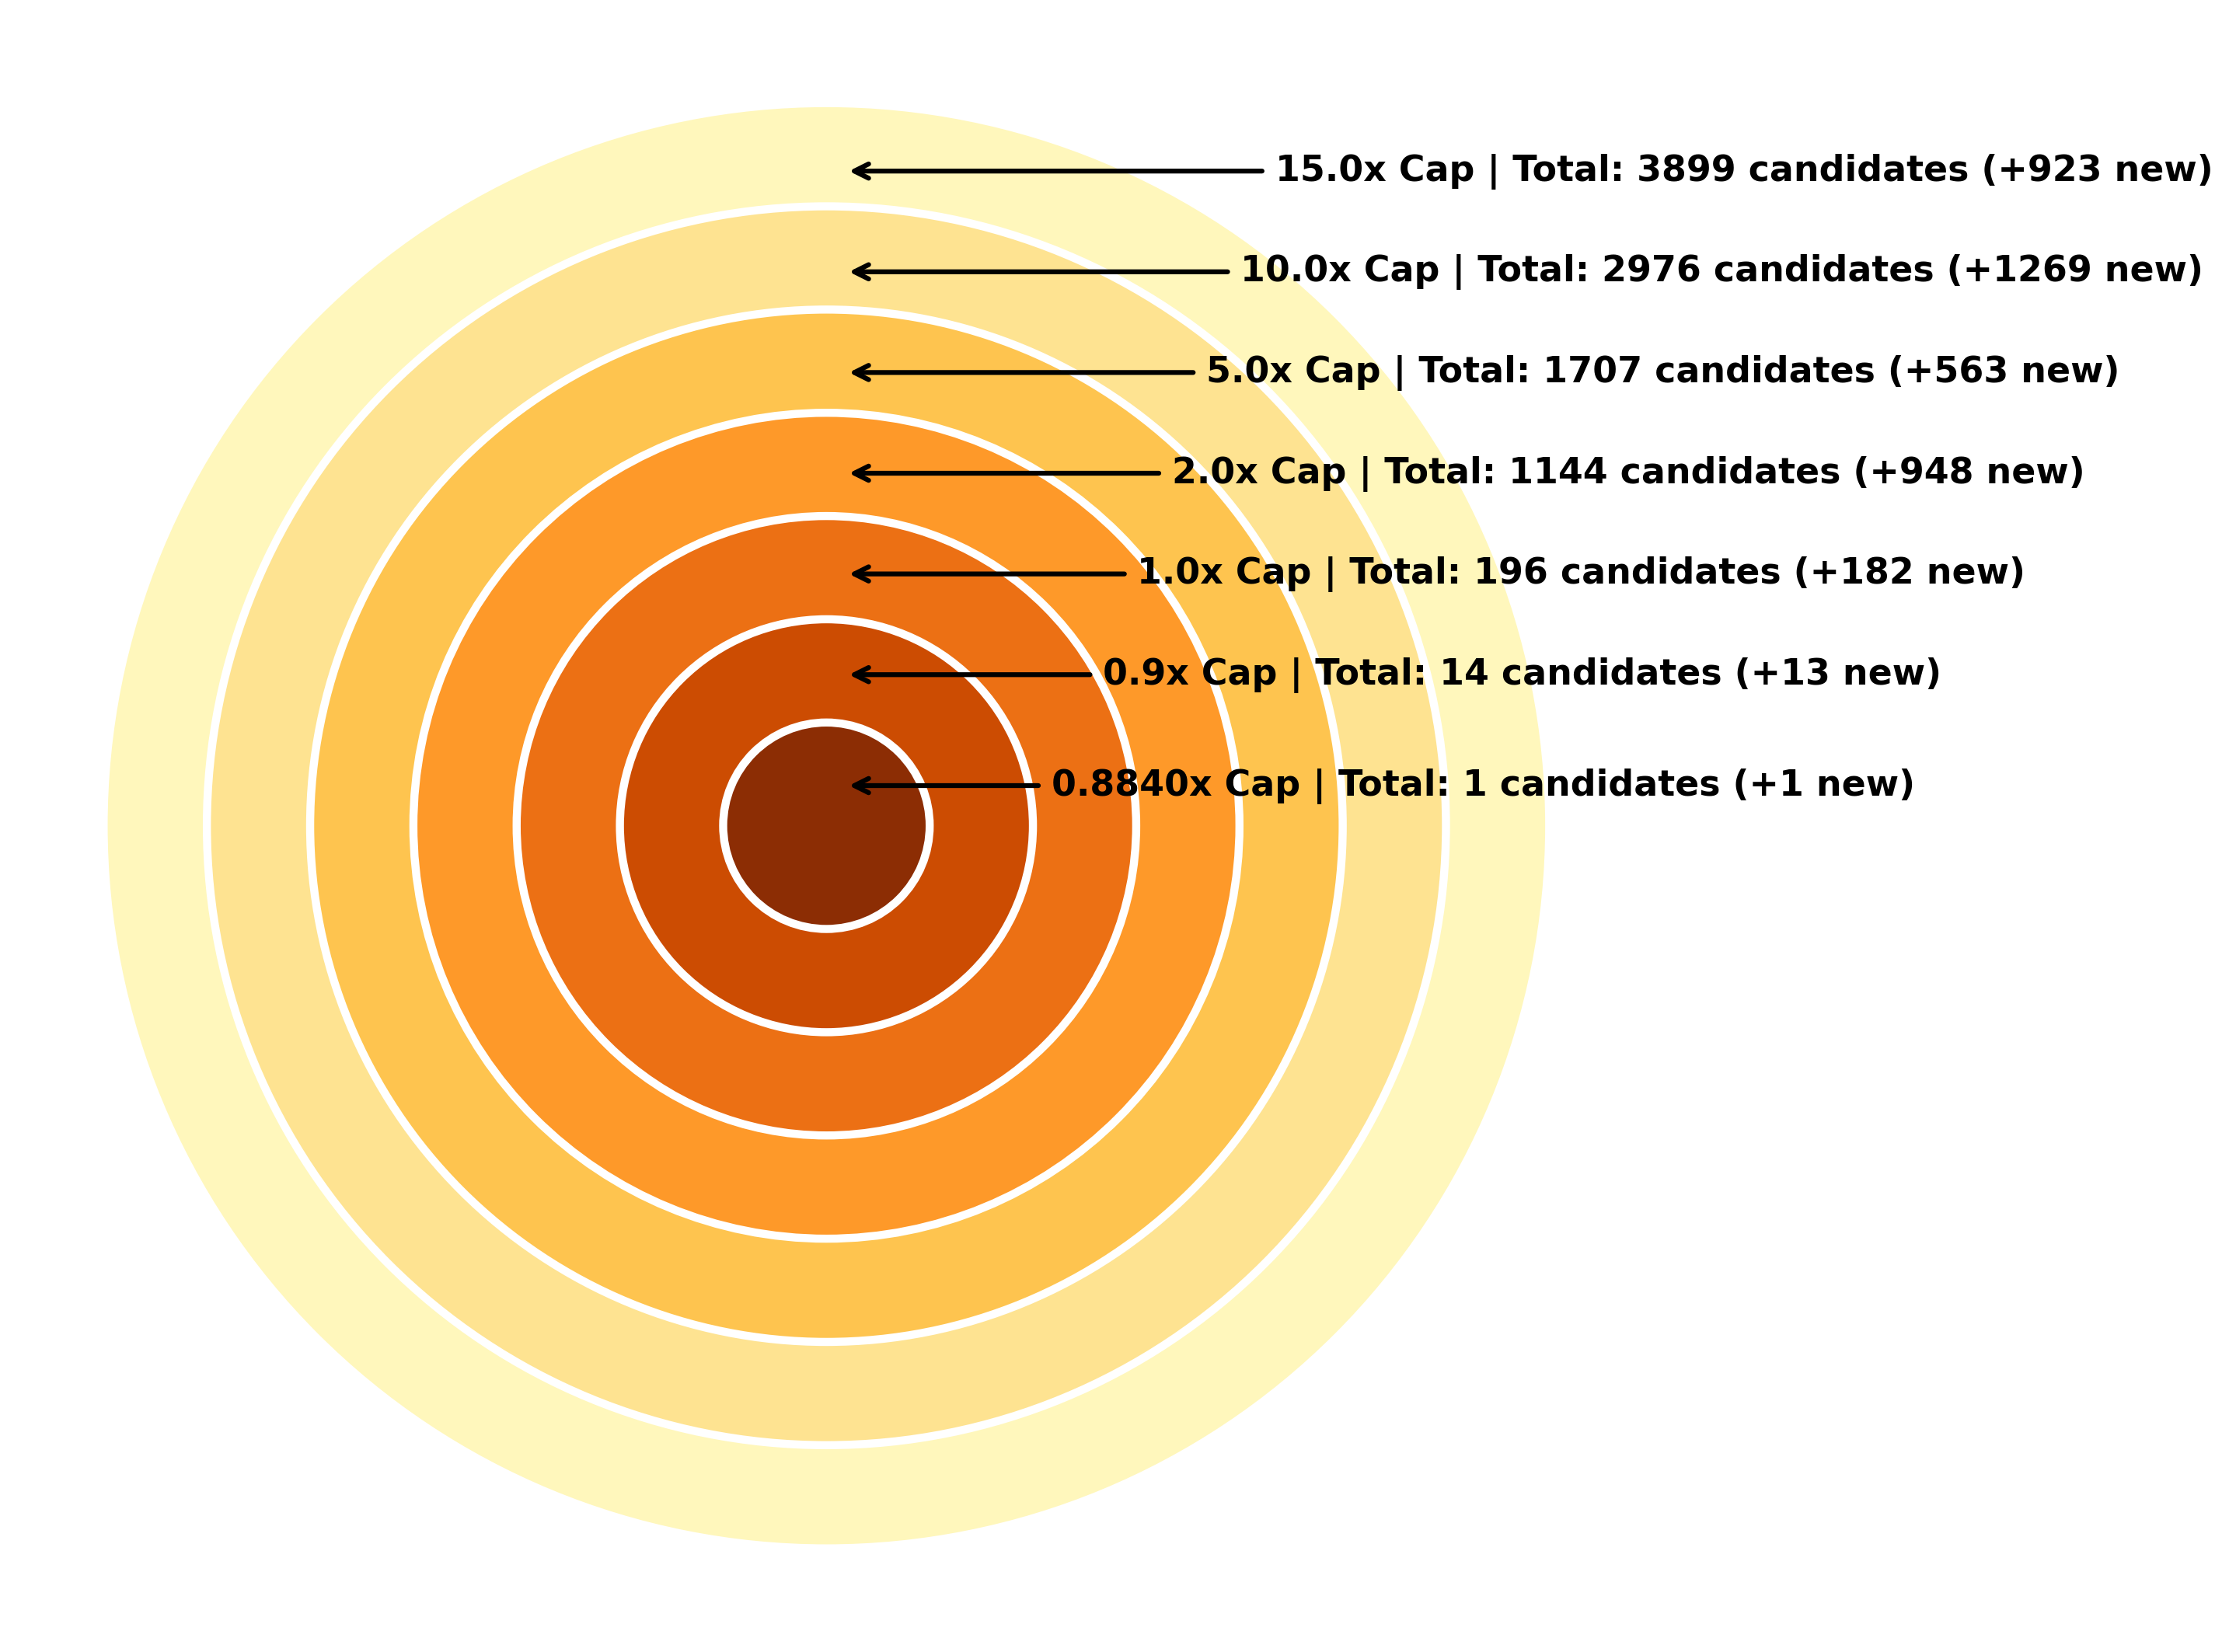
\includegraphics[width=0.5\textwidth]{content/images/concentric_diagram.png}
    \caption{Global Minimax Expansion: Concentric Euler diagram illustrating the volume of candidates unlocked at expanding uniform multiplier thresholds.}
    \label{fig:concentric_minimax}
\end{figure}

Obviously, the smaller the multiplier $X$, the smaller number of candidates we get through the search process. Moreover, we can see a clear winner ($X \approx 0.8840$), but let's investigate how cool it is (Table~\ref{tab:optimal_candidate_metrics}). 

\begin{table}[h!]
    \centering
    \small
    \caption{Performance Comparison between the Standard Baseline and the Balanced Candidate}
    \label{tab:optimal_candidate_metrics}
    \begin{tabular}{lrrr}
        \toprule
        \textbf{Metric} & \textbf{Standard Baseline} & \textbf{Optimal Candidate} & \textbf{Ratio} \\
        \midrule
        Parameters $(h, d, k, a, w)$ & $(63, 7, 14, 12, 16)$ & $(40, 5, 24, 8, 16)$ & -- \\
        Signature Size (Bytes) & $7,872$ & $6,928$ & $0.8801\times$ \\
        Key Generation Cost & $292,862.0$ & $146,430.0$ & $0.5000\times$ \\
        Signing Cost & $2,279,391.0$ & $756,689.0$ & $0.3320\times$ \\
        Verification Cost & $2,387.0$ & $1,857.0$ & $0.7780\times$ \\
        Compression per Byte ($\rho$) & $0.303227$ & $0.268043$ & $0.8840\times$ \\
        \bottomrule
    \end{tabular}
\end{table}

Someone can say it's pretty good. Our opinion that 12\% win on the signature size isn't very attractive. 

\paragraph{Optimal Search Strategy} Every candidates can be related to the some tuple of metrics value. 
The search for optimal candidate could be represented as finding the closest point to the origin in five dimentionl space (finding the shortest vector). 
The issue is that we cannot visualize the such high dimentional space, but we can analyse the 2D projections of 5 dimentional space.
We could create 10 graphs of every metrics pairs, but It is quite complicated to analyse.
The better option is the strategy, were we define the metrics that are important to us, and the rest we cound use the default filter, by setting $X=1$. 
And to find the best candidate, we serach for the point that the the closest to the origin.

Let's see the the visualized example below, where we chose signature size and signing cost as important metrics, while other must be better than the baseline.

\begin{figure}[htbp]
    \centering
    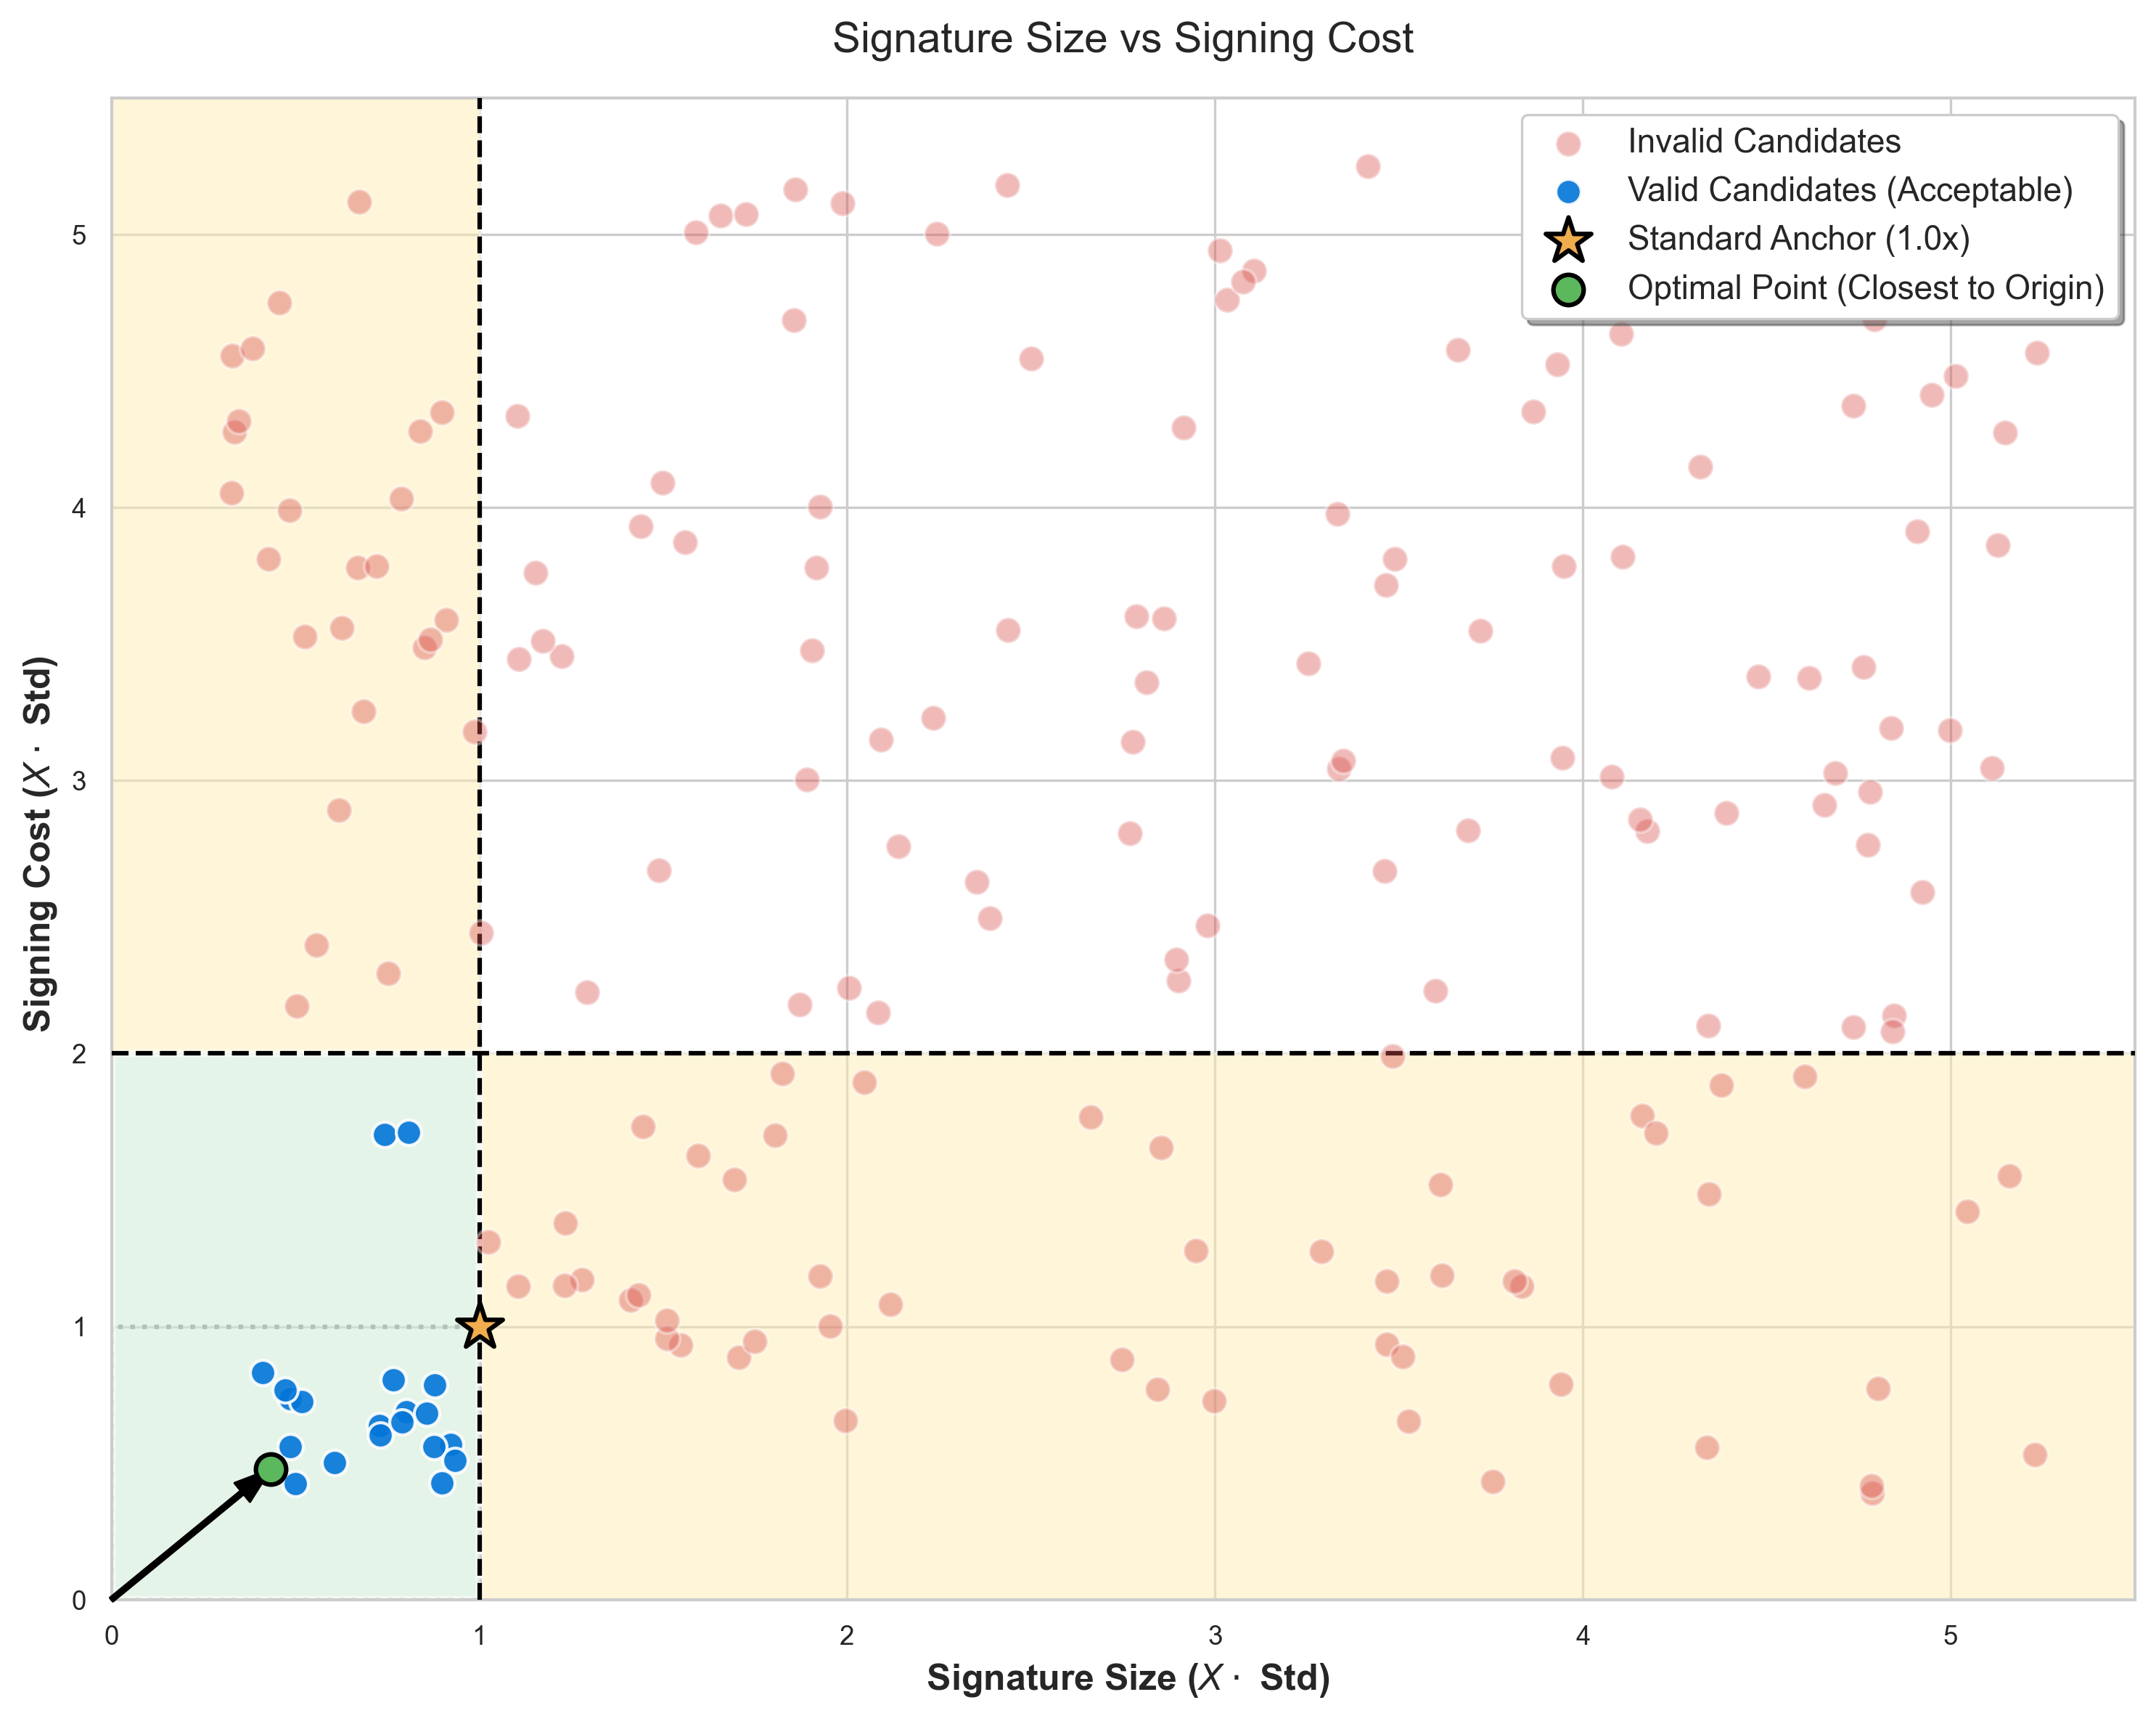
\includegraphics[width=0.8\textwidth]{content/images/scatter_plot.png}
    \caption{Visualization of Candidates with Prioritization of Size and Signing Cost Metrics.}
    \label{fig:scatter_plot}
\end{figure}

While this interpretation of the parameters search fulfills its purpose to demonstrate how actually we find the candidates, this method needs more plots to know the exact values.
We can do better! 

In the new strategy, we plot unbounded parameters set (with only condition to have 128 bits security) on the plane randomly (the position doesn't matter). 
After initializing candidates, apply the signature size filter, visualized as color filtering card. Moving further apply all other filter unil the last one.
The resulting set is the set with appropriate candidates where we can search for the best. 

Let's consider an example, where we set the following coefficients in the filters: 
$$X_{\text{size}} = 0.85, X_{\text{kg}} = 1.5, X_{\text{sg}} = 2, X_{\text{sv}} = 0.8, X_{\text{cb}} = 1.$$

The result of search for candidates with filtering shown below (see the Figure~\ref{fig:full_filtering_process}):

\begin{figure}[htbp]
    \centering
    % Row 1
    \begin{subfigure}[b]{0.32\textwidth}
        \centering
        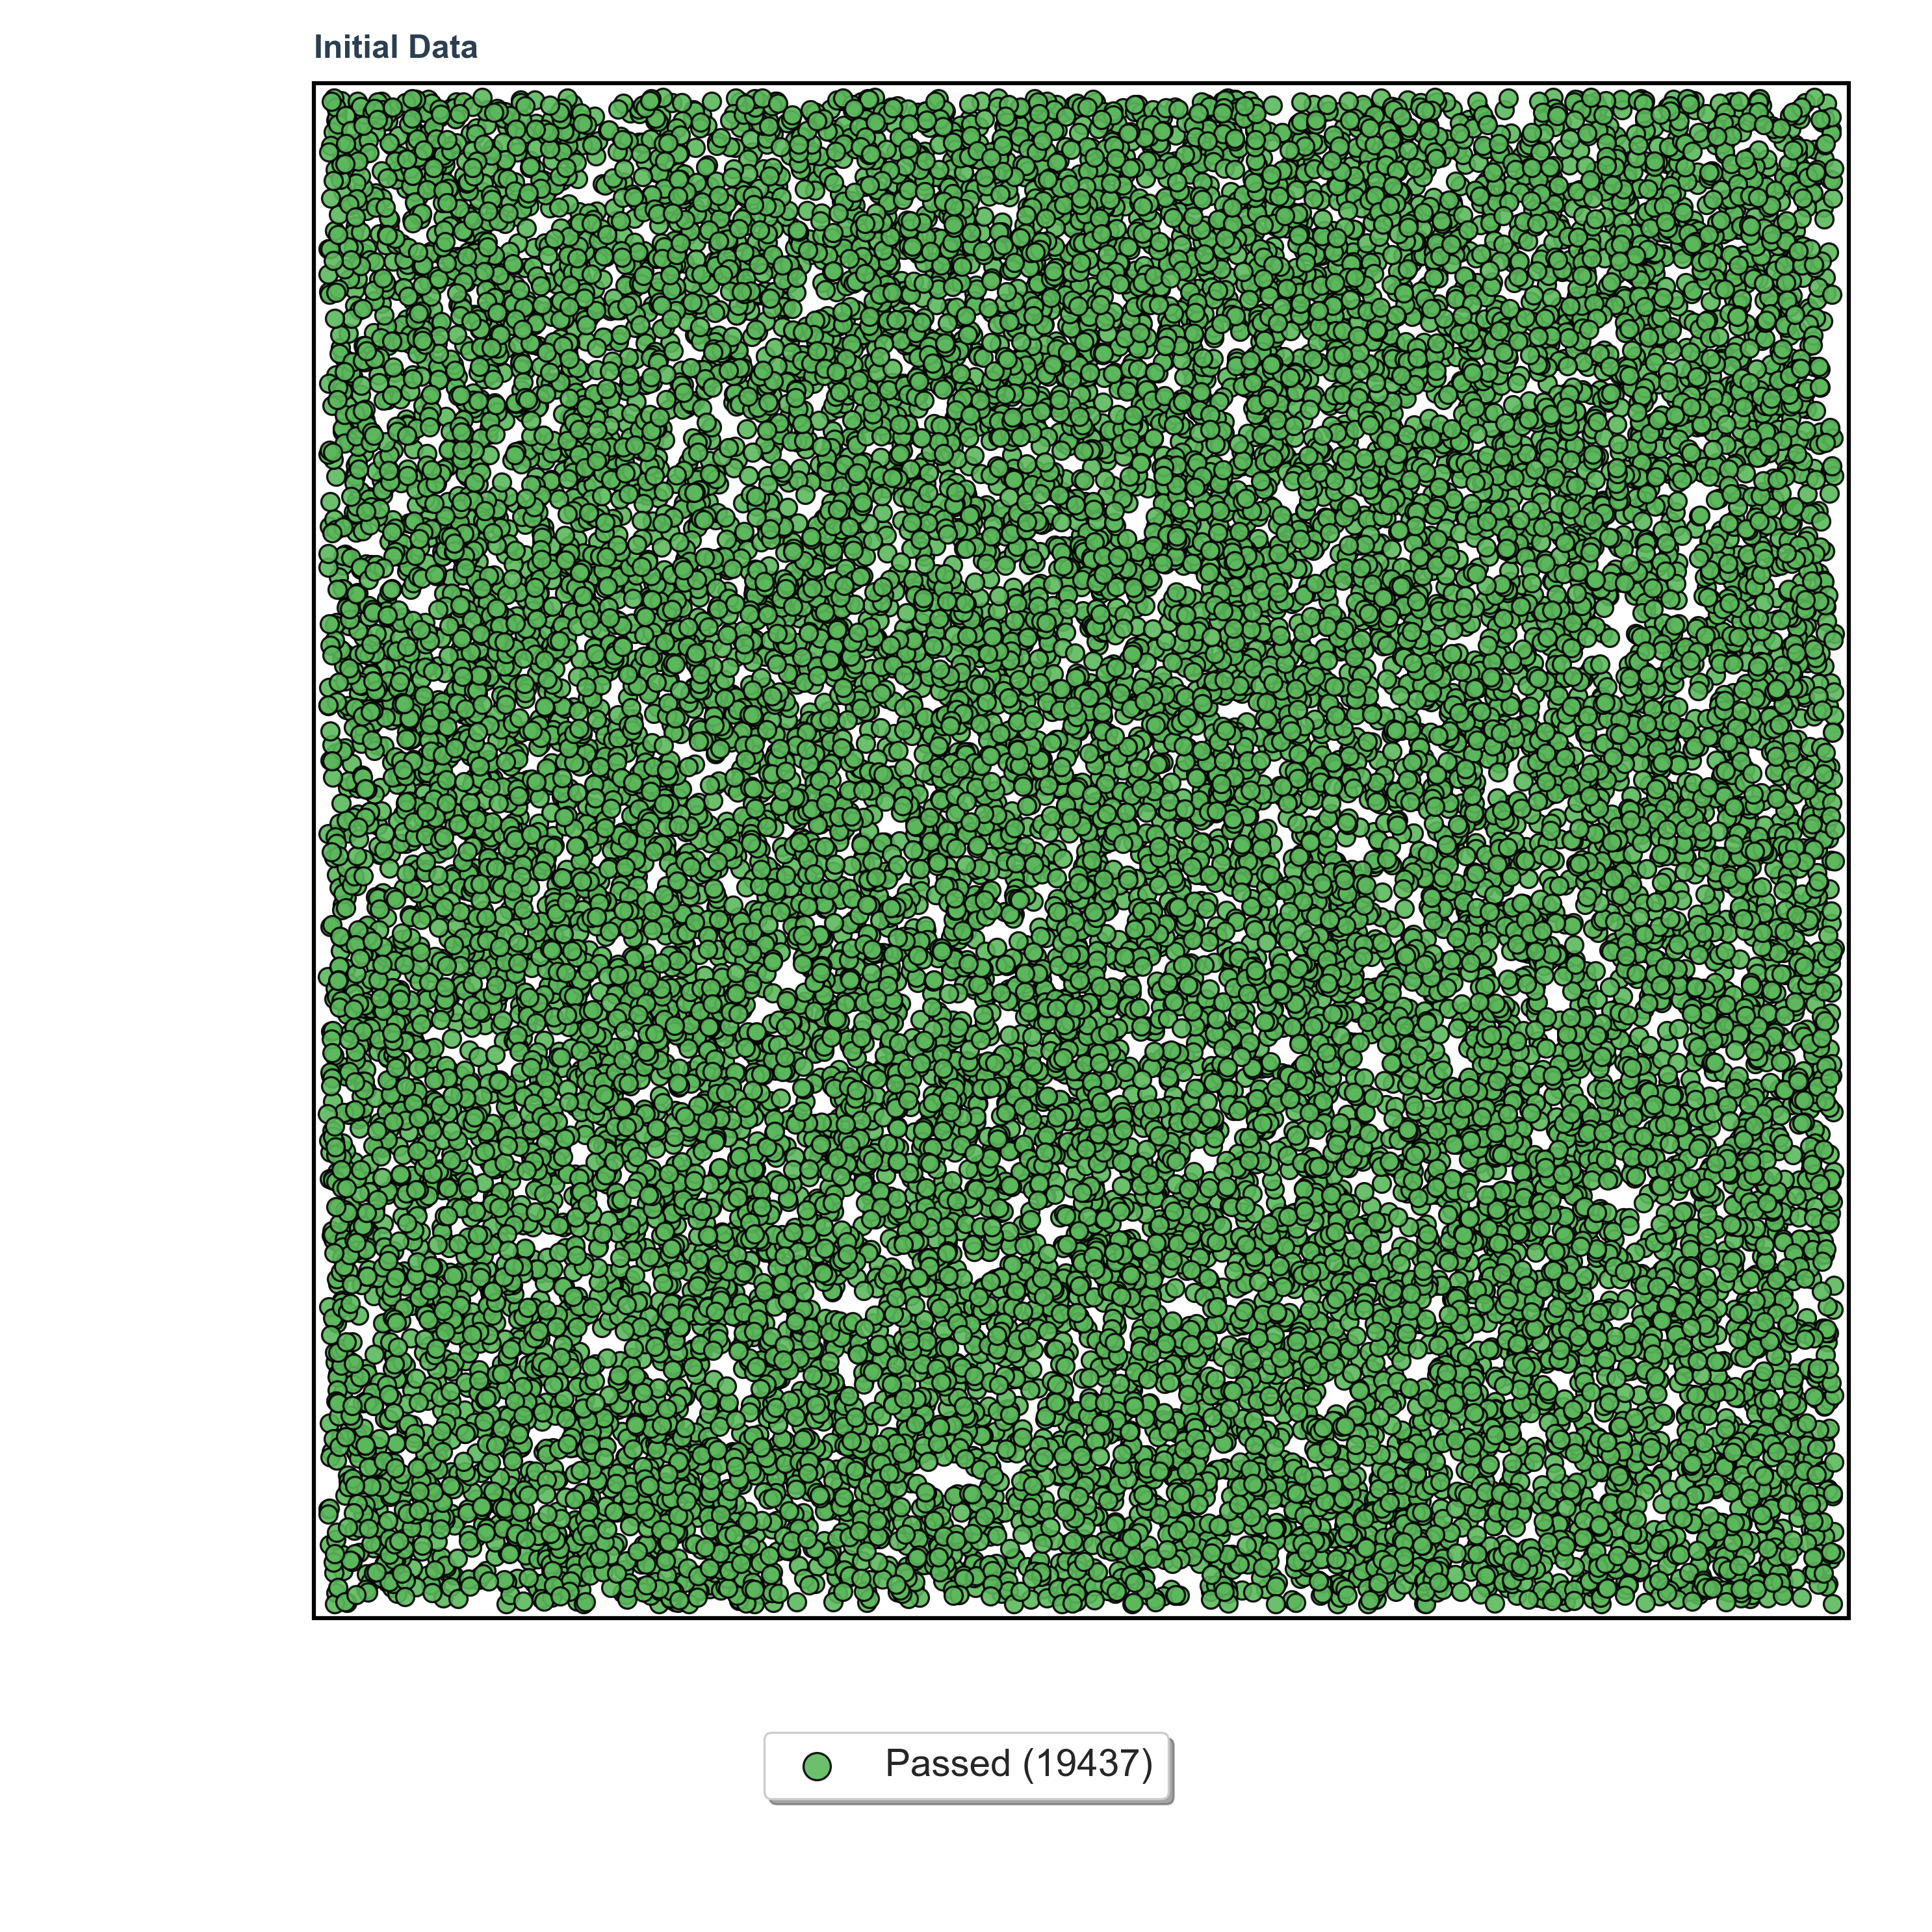
\includegraphics[width=\textwidth]{content/images/sieve_step1_initial.png}
        \caption{Initial Pool}
        \label{fig:sieve_1}
    \end{subfigure}
    \hfill
    \begin{subfigure}[b]{0.32\textwidth}
        \centering
        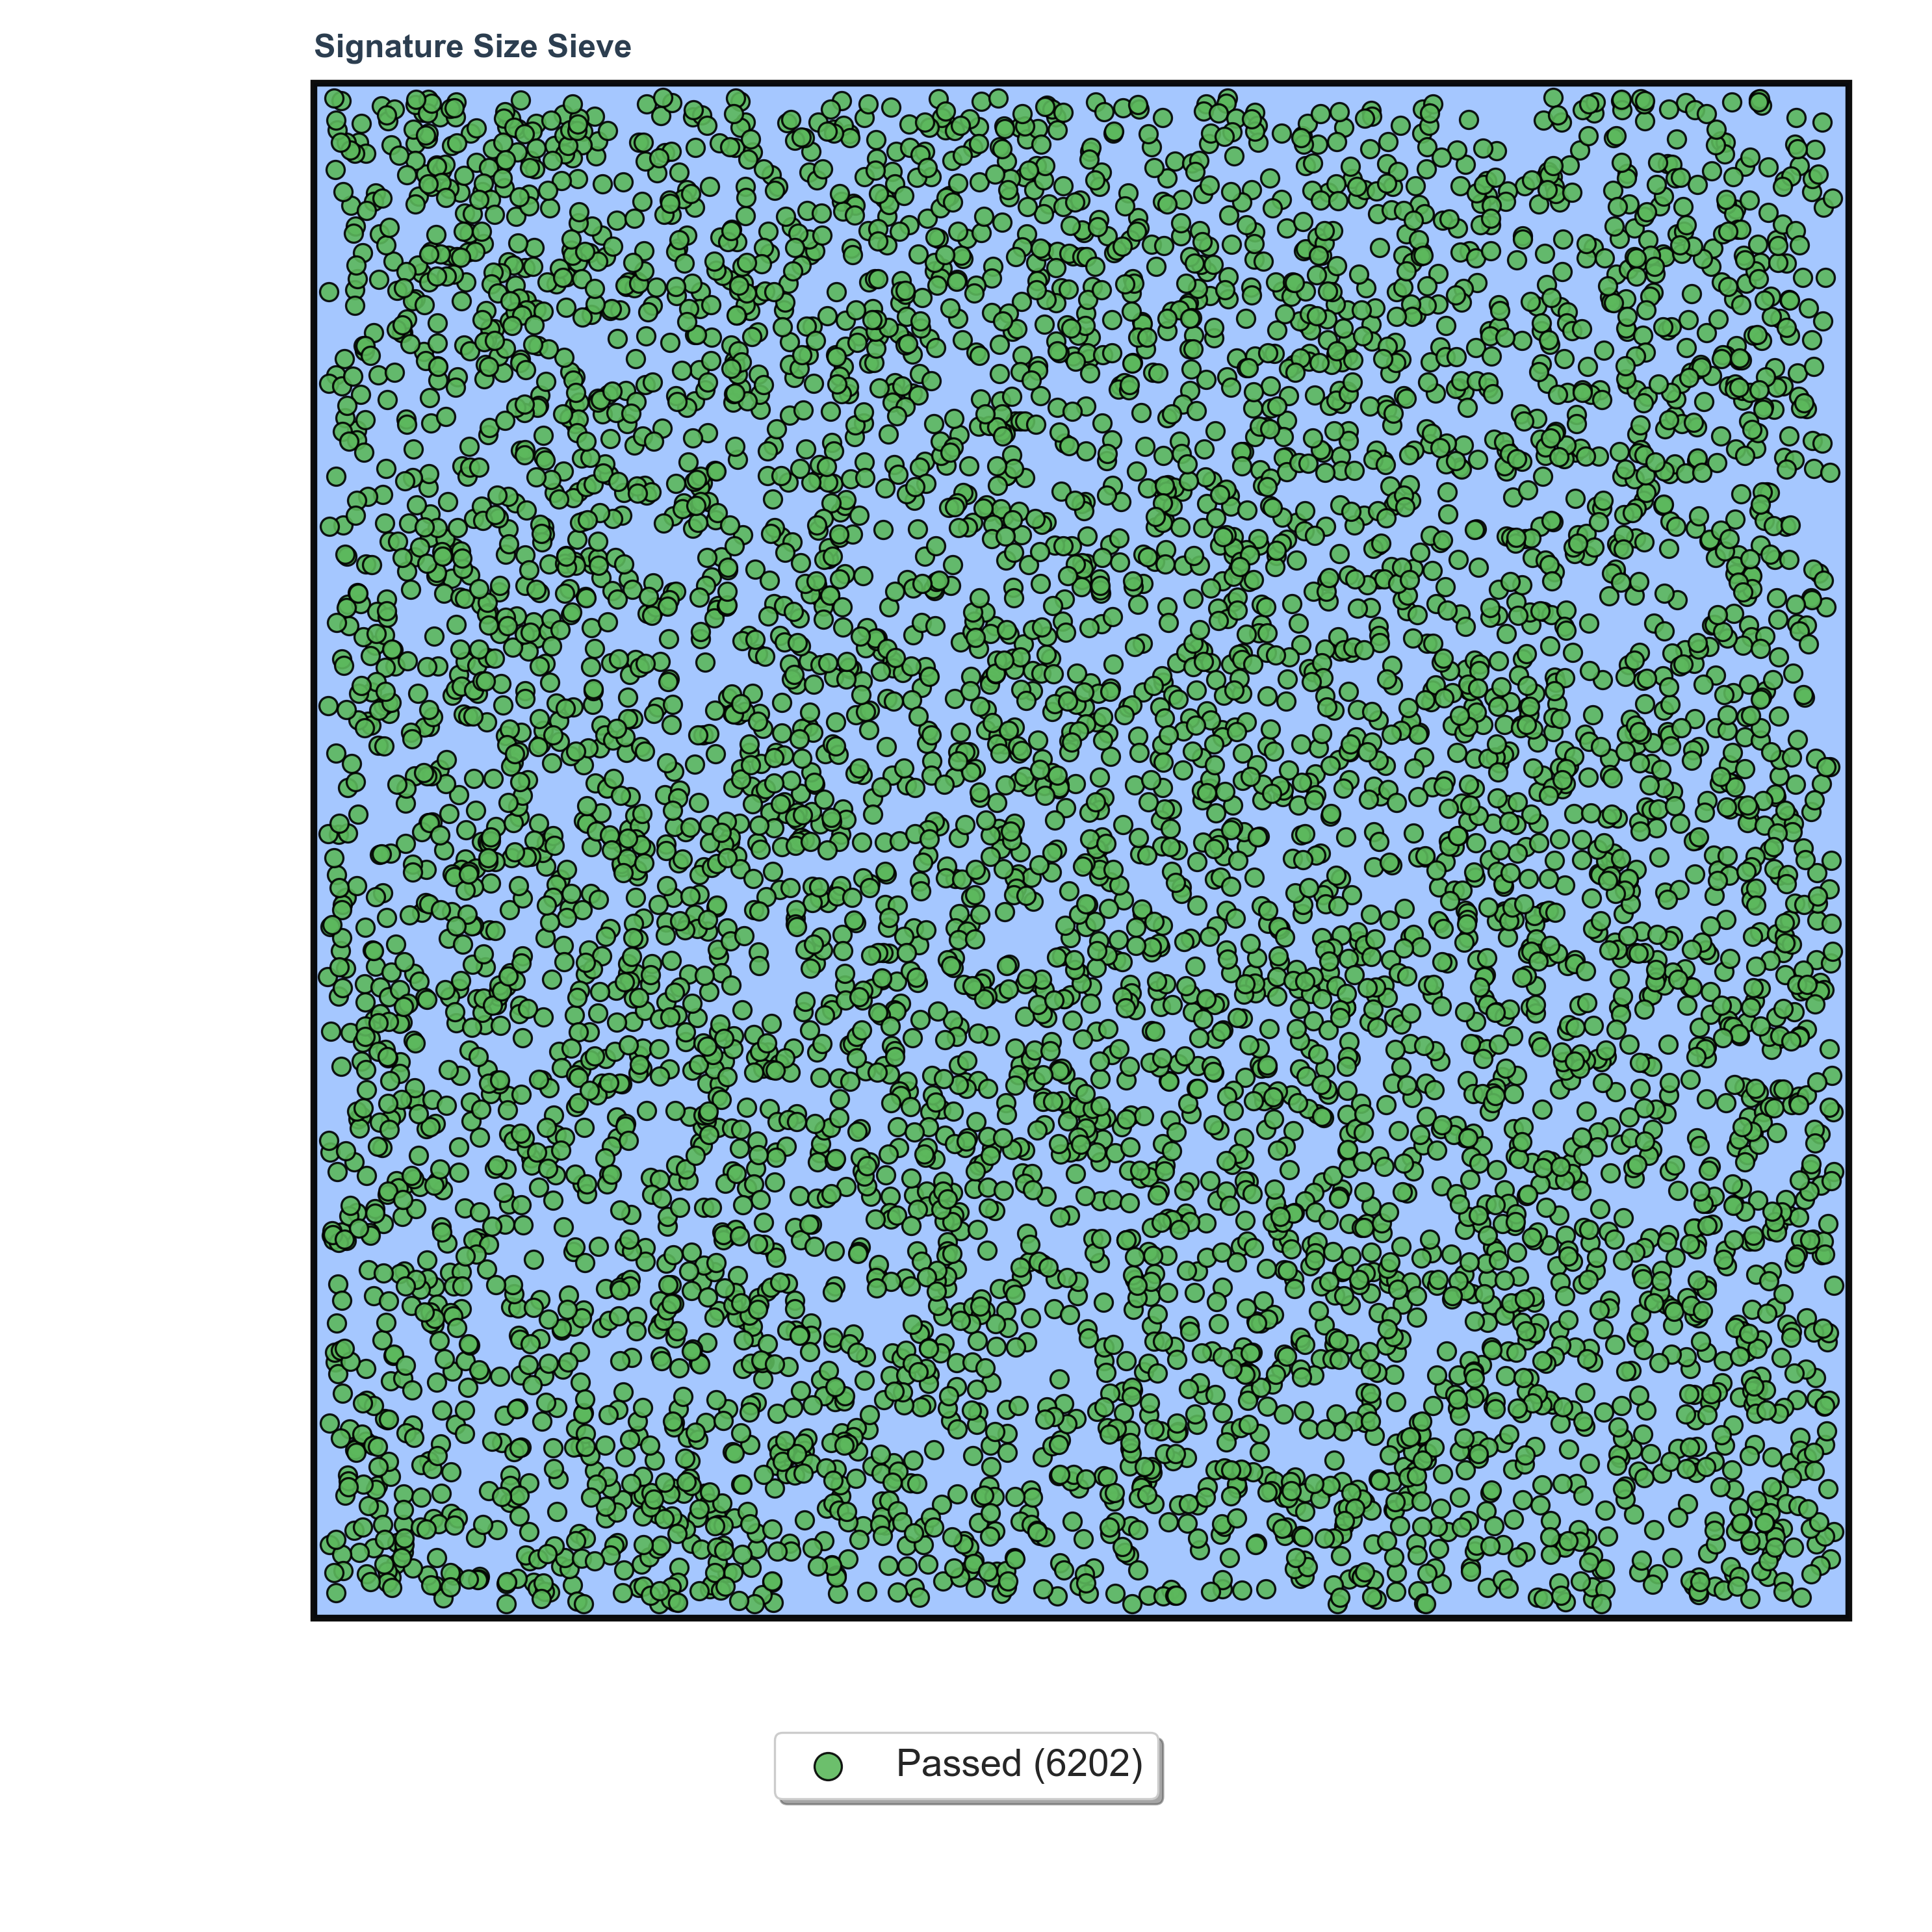
\includegraphics[width=\textwidth]{content/images/sieve_step2_size.png}
        \caption{SigSize}
        \label{fig:sieve_2}
    \end{subfigure}
    \hfill
    \begin{subfigure}[b]{0.32\textwidth}
        \centering
        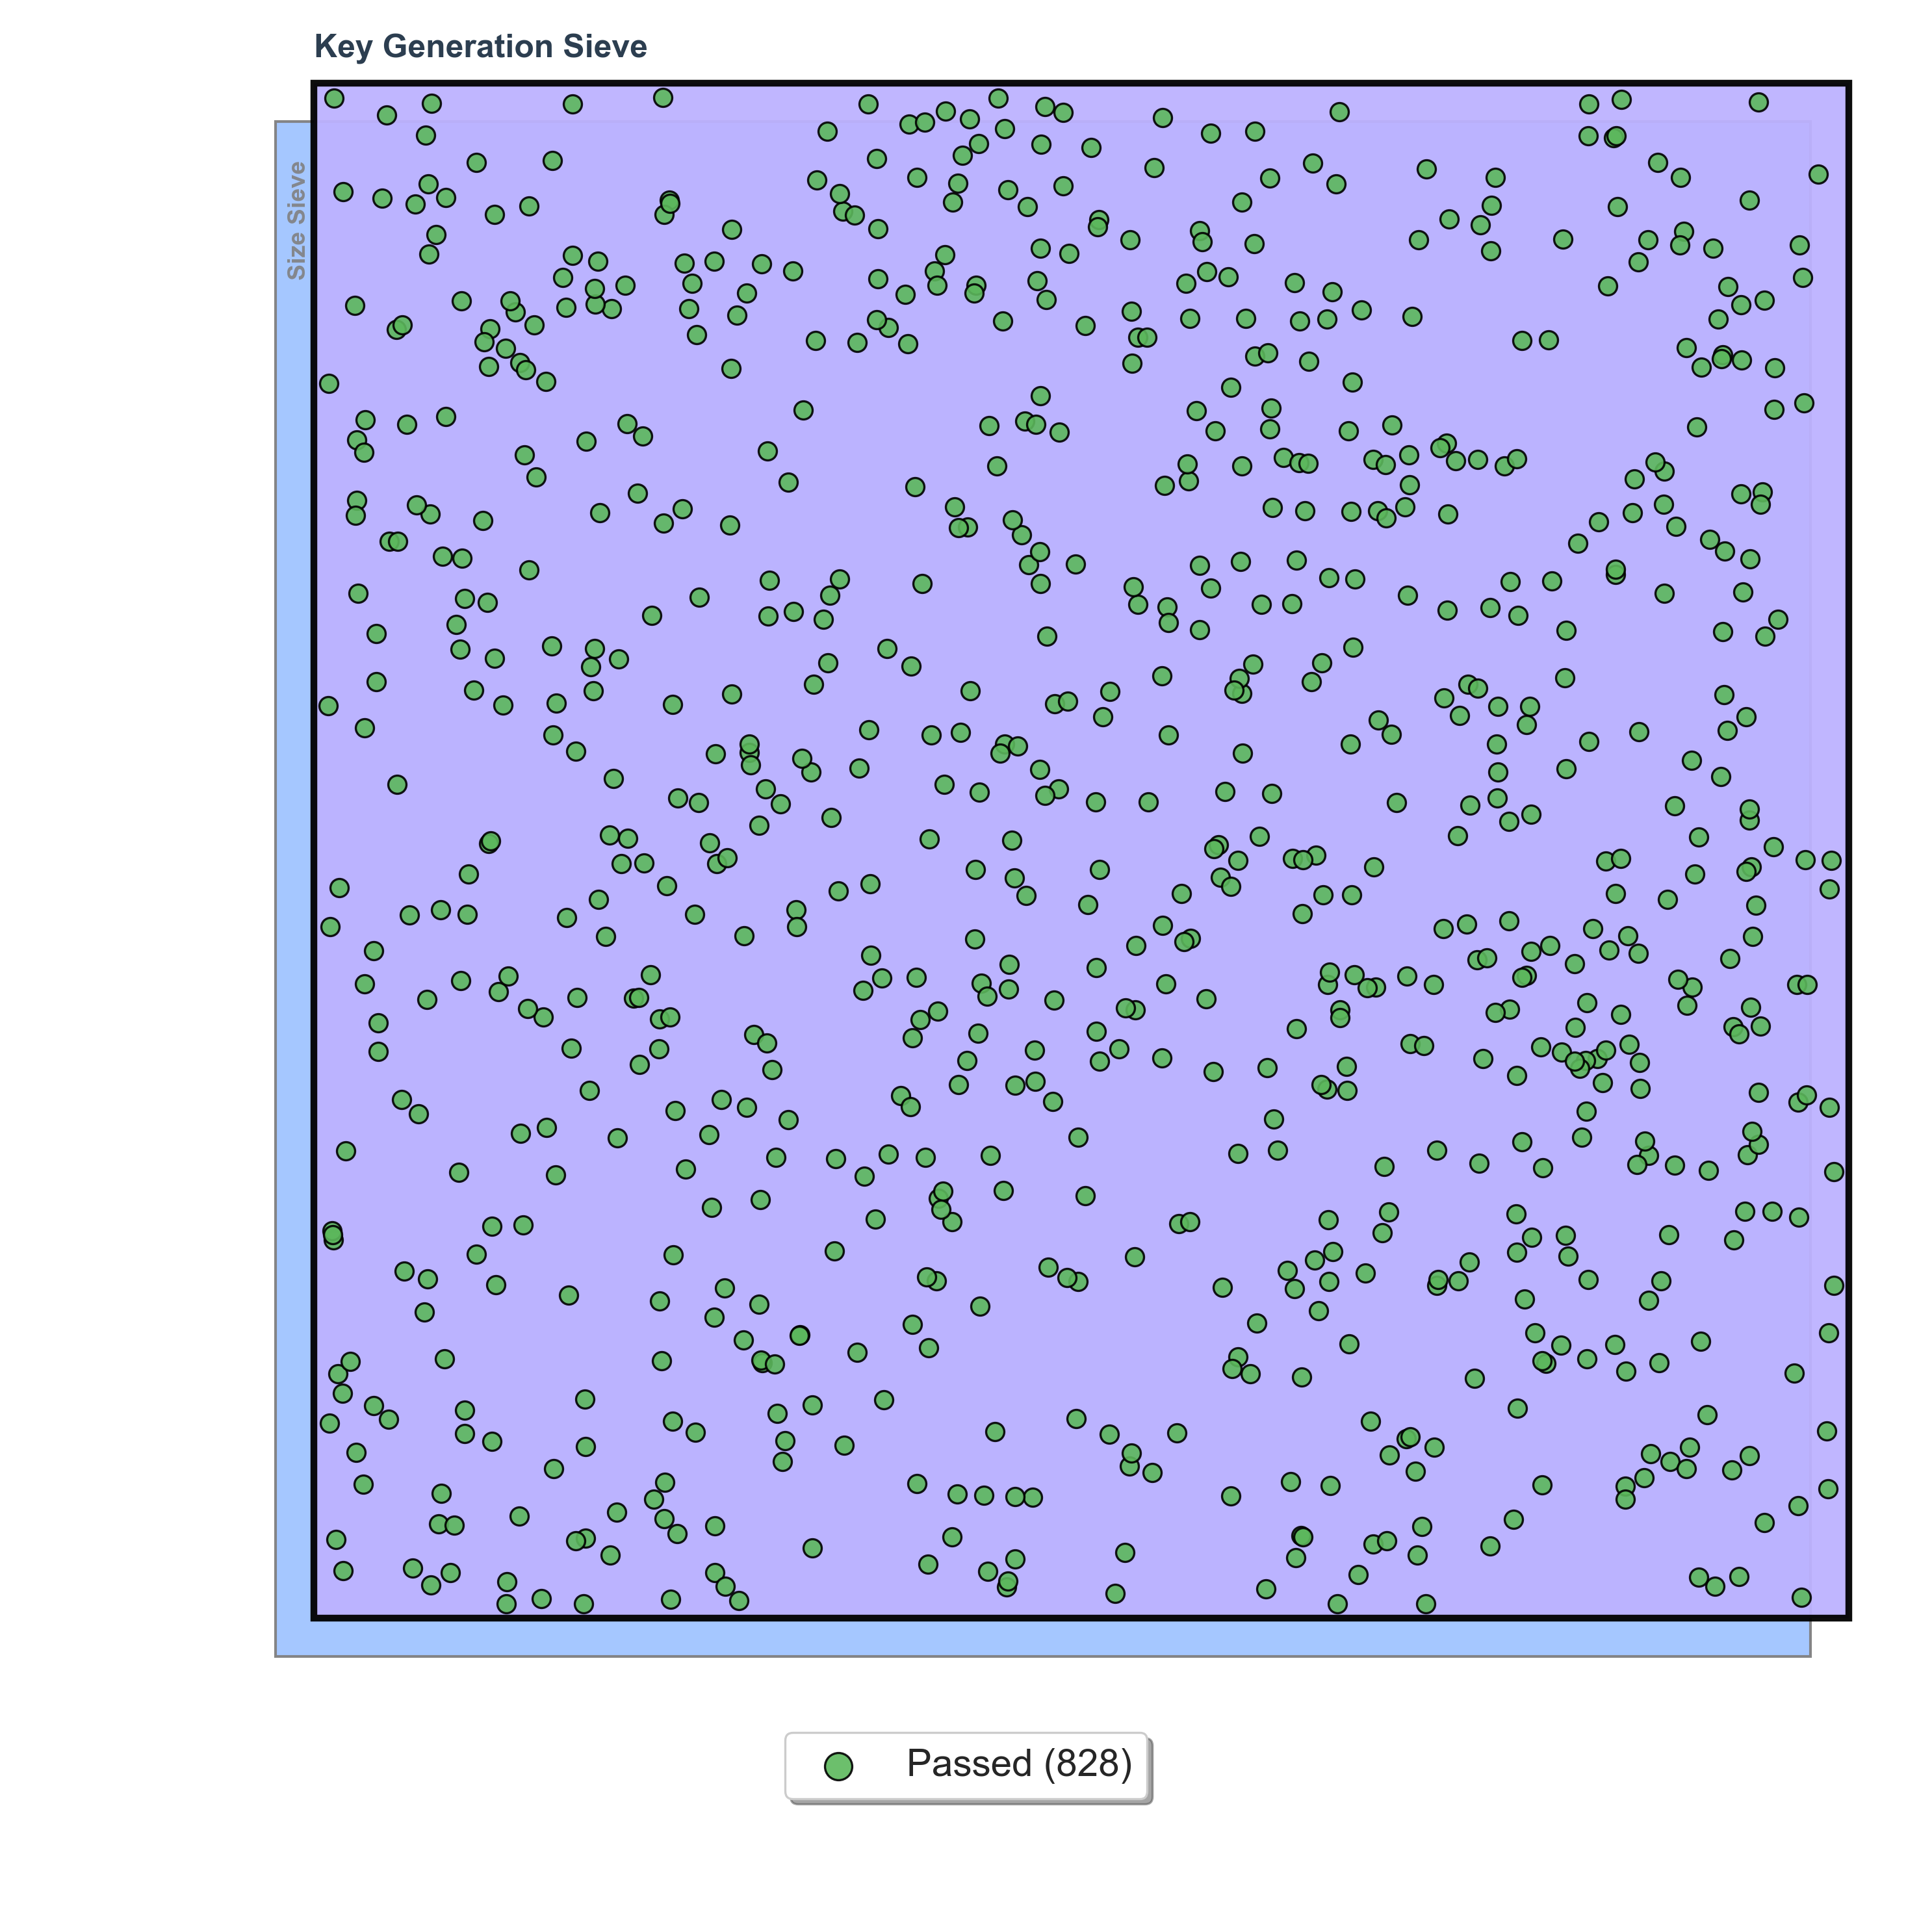
\includegraphics[width=\textwidth]{content/images/sieve_step3_keygen.png}
        \caption{KeyGen}
        \label{fig:sieve_3}
    \end{subfigure}
    
    \vspace{0.5cm}
    
    % Row 2
    \begin{subfigure}[b]{0.32\textwidth}
        \centering
        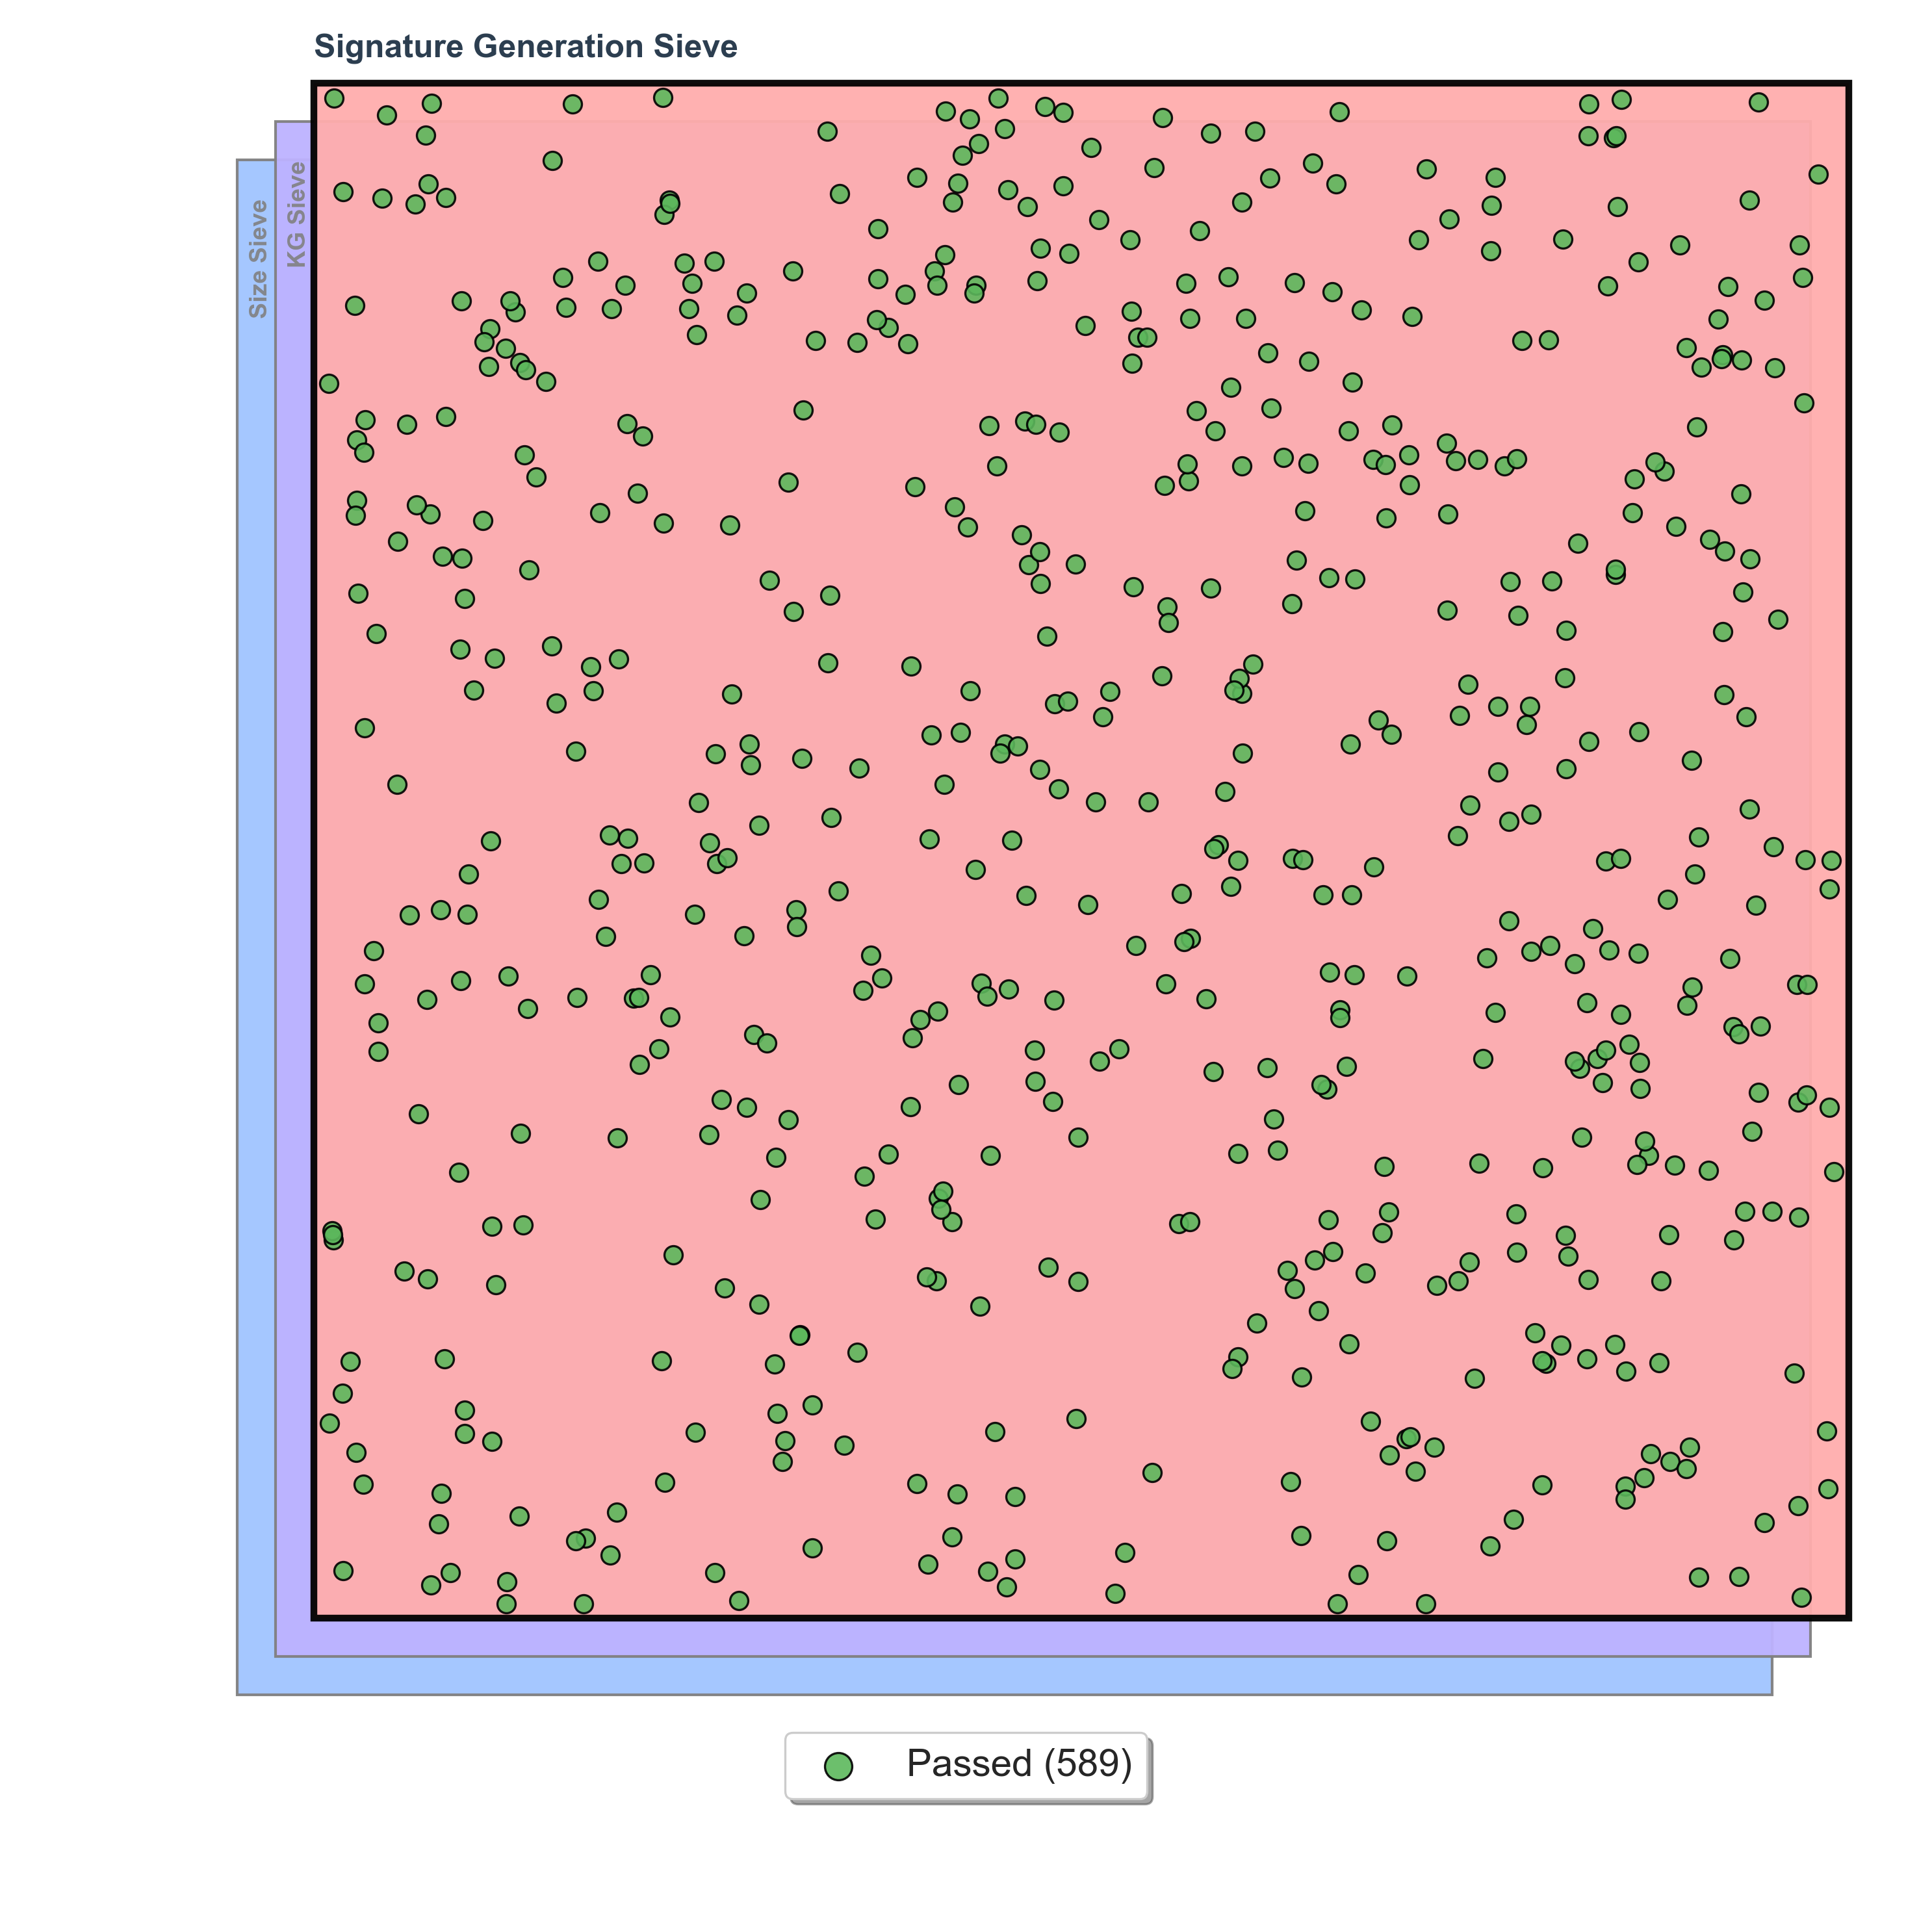
\includegraphics[width=\textwidth]{content/images/sieve_step4_siggen.png}
        \caption{SigGen}
        \label{fig:sieve_4}
    \end{subfigure}
    \hfill
    \begin{subfigure}[b]{0.32\textwidth}
        \centering
        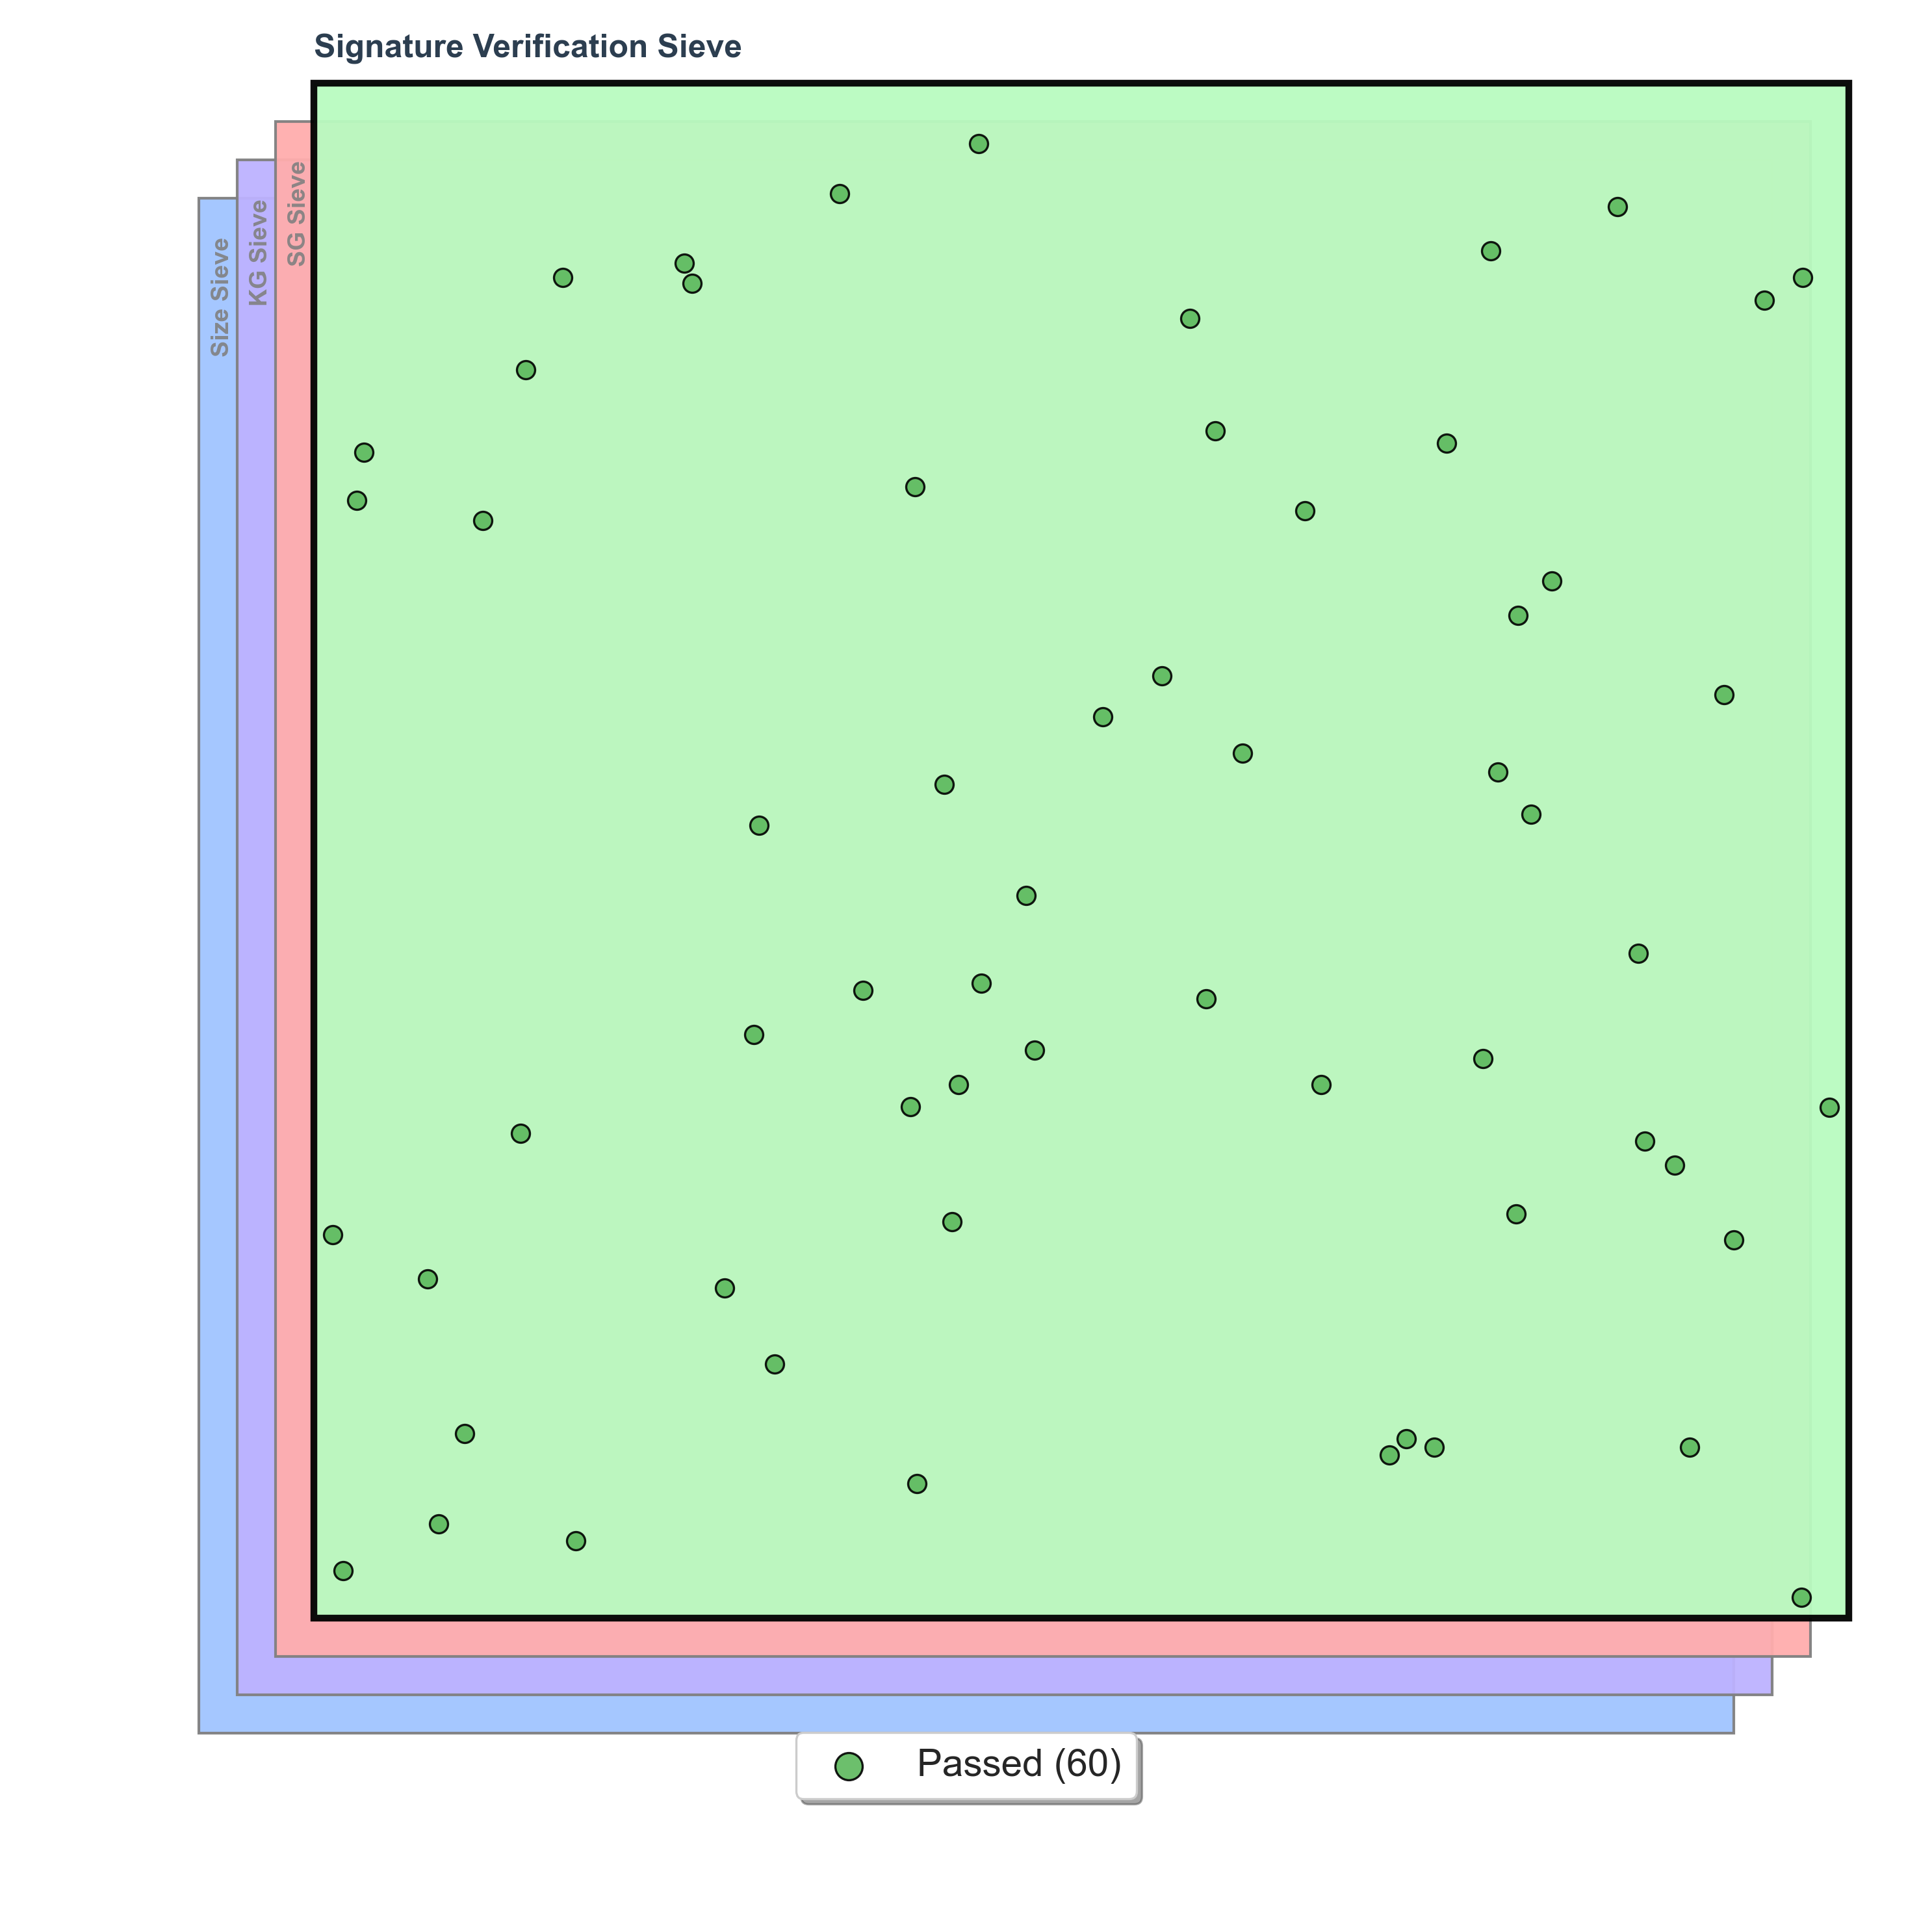
\includegraphics[width=\textwidth]{content/images/sieve_step5_verify.png}
        \caption{SigVerify}
        \label{fig:sieve_5}
    \end{subfigure}
    \hfill
    \begin{subfigure}[b]{0.32\textwidth}
        \centering
        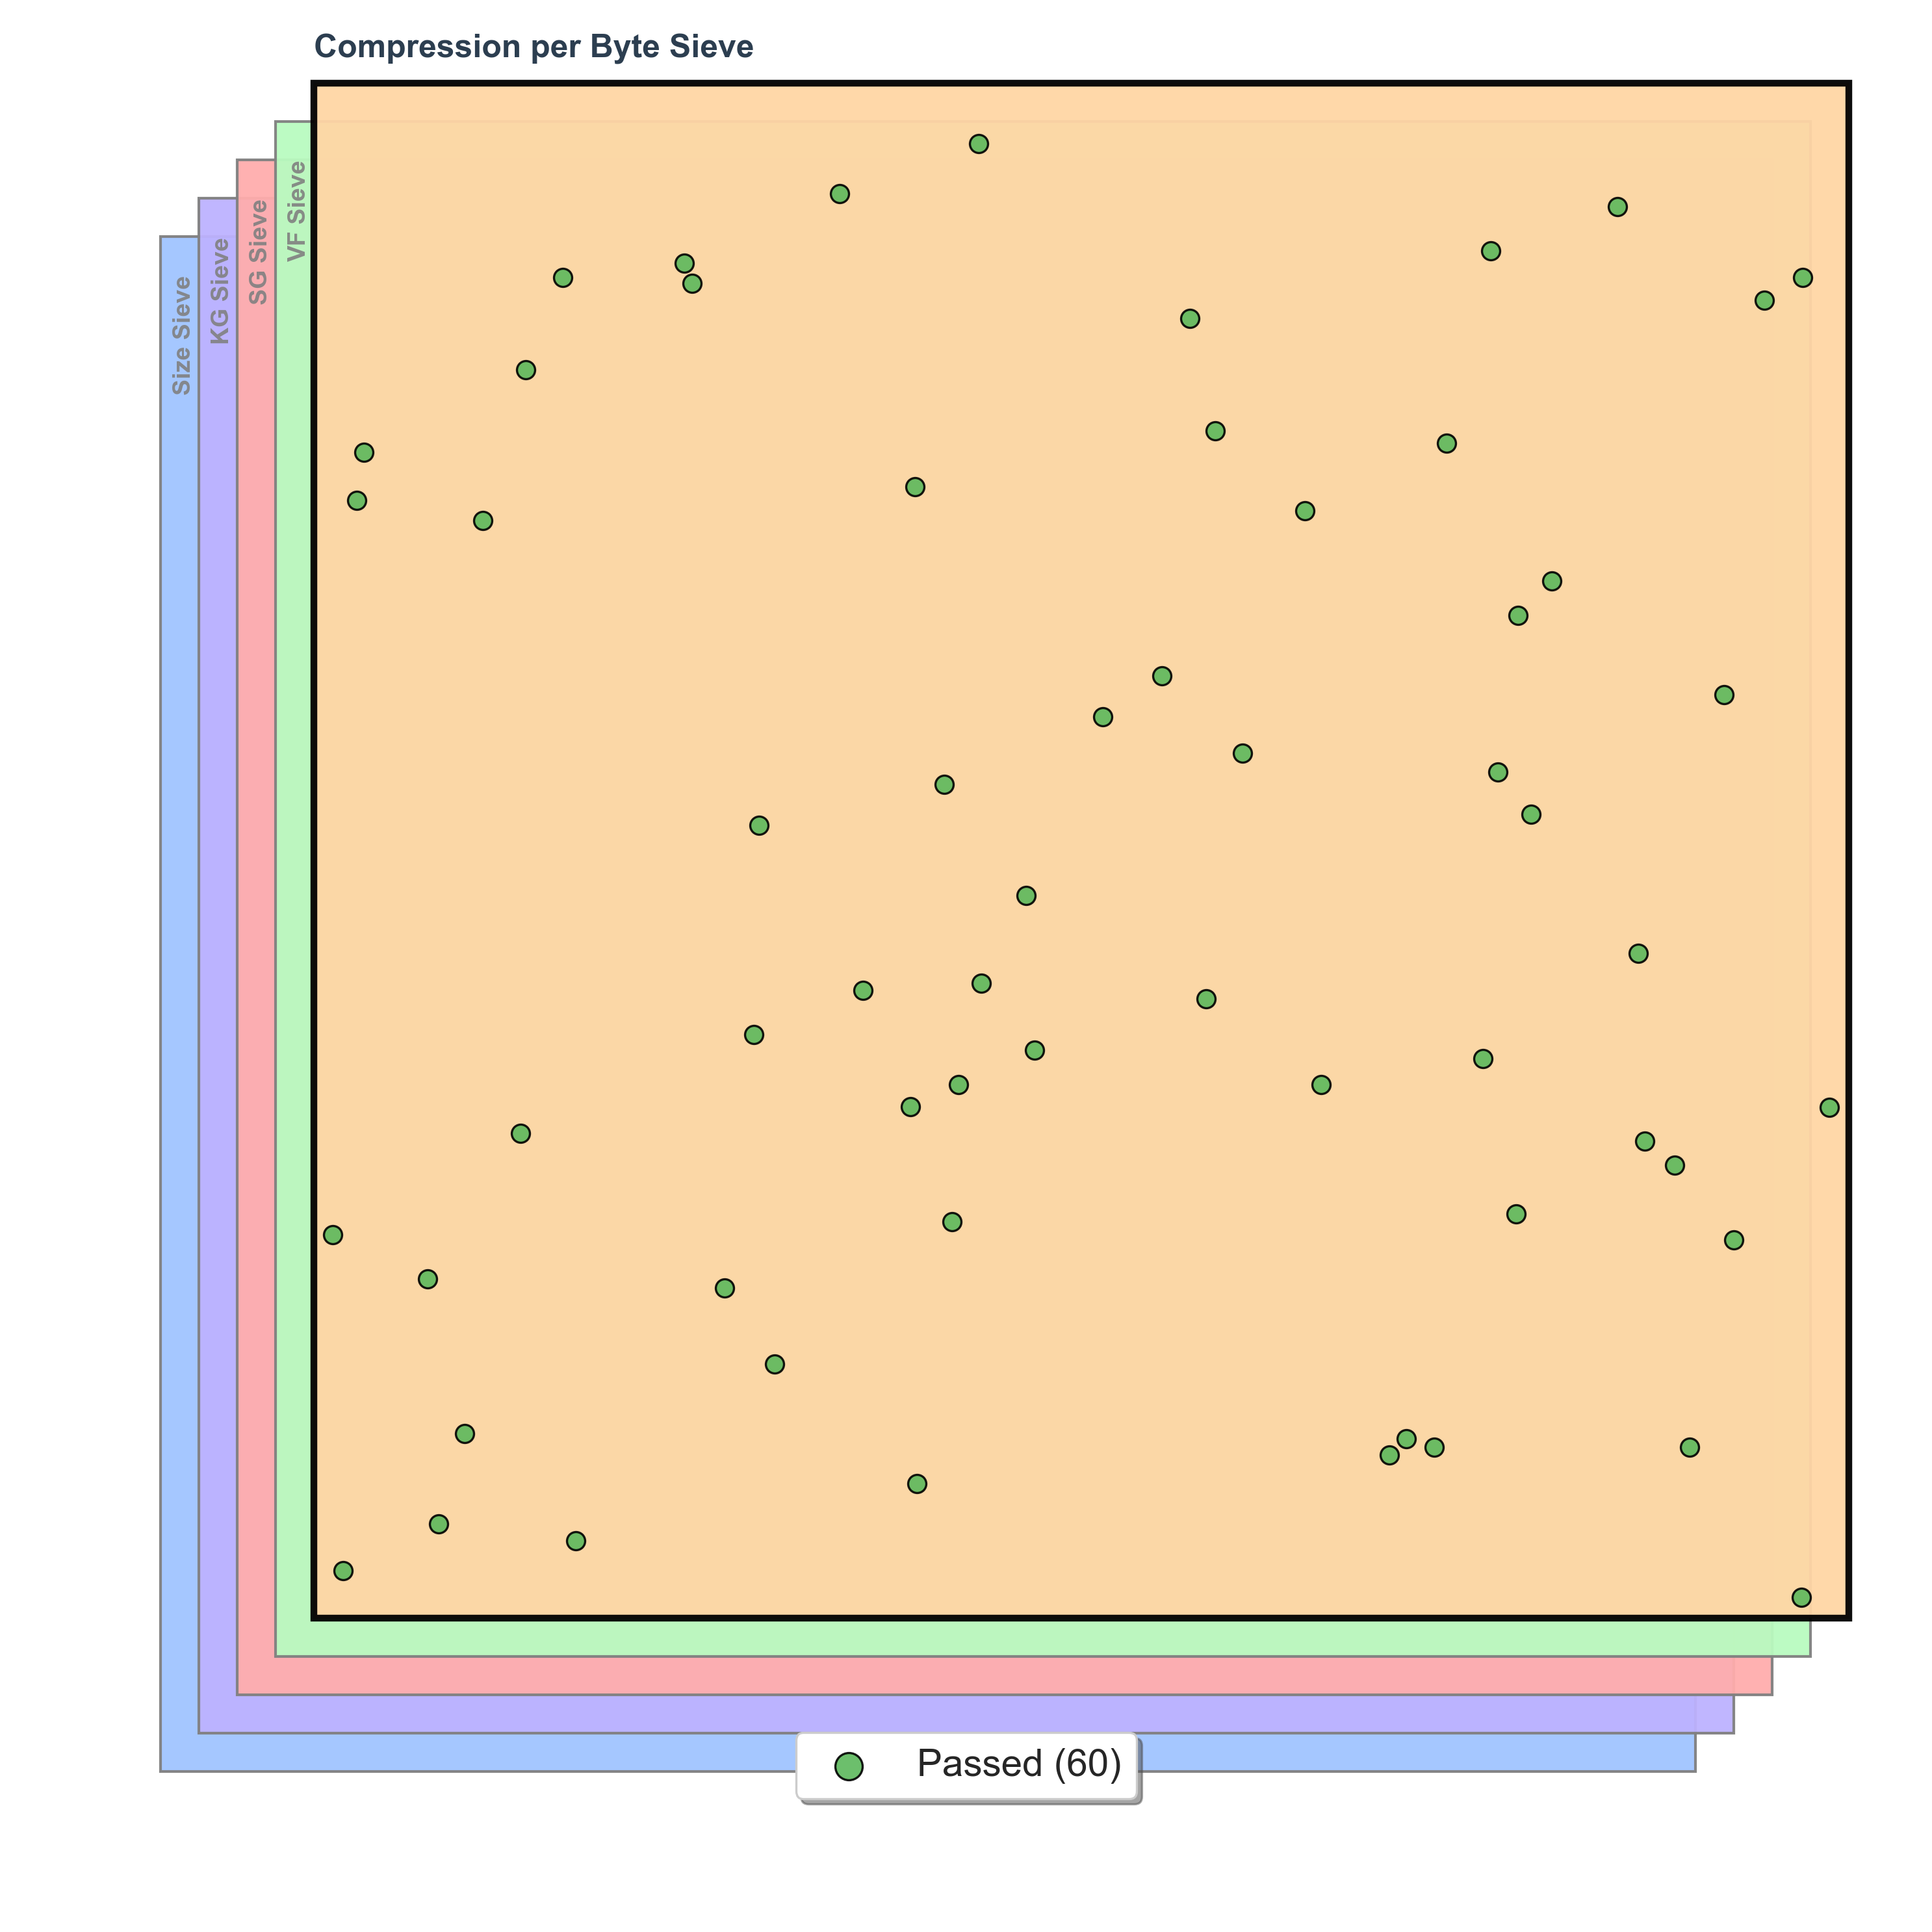
\includegraphics[width=\textwidth]{content/images/sieve_step6_rho.png}
        \caption{Comp/Byte}
        \label{fig:sieve_6}
    \end{subfigure}
    
    \caption{Full Parameter Filtering Process}
    \label{fig:full_filtering_process}
\end{figure}

Starting with the total number of candidates equal to 19437. After applying signature size filter, succesfully reduce the number of candidates up to 6202.
In the next step, we reduce the candidates in more than 7 times. 
Filtering further, we left with smaller and smaller number of suitable candidates, resulting only in final 60 candidates to check further. 

Obtaining the set of final candidates, we are ready to search for the best among them. 
For this part we use weighted euclidean distance. 
The reason behind choosing such metric lies in the ability to sign the priority of metrics.
Let's define the raw weight coefficients as $w_{\text{size}}, w_{\text{kg}}, w_{\text{sg}}, w_{\text{sv}}$, and $w_{\text{cb}}$, representing the relative priority of signature size, key generation, signing, verification, and compression per byte, respectively. All coefficients are real positive numbers ($w \in \mathbb{R}^+$). 

To ensure the calculation remains proportionally consistent regardless of the scale of the chosen weights, we normalize them into coefficients $p_i$ (where $i \in \{\text{size}, \text{kg}, \text{sg}, \text{sv}, \text{cb}\}$) such that their total sum equals $1$:
\begin{equation}
    p_i = \frac{w_i}{w_{\text{size}} + w_{\text{kg}} + w_{\text{sg}} + w_{\text{sv}} + w_{\text{cb}}}, \quad \text{ensuring} \quad \sum p_i = 1
    \label{eq:weight_normalization}
\end{equation}

Using these normalized coefficients, we calculate the Weighted Euclidean Distance (the $L_2$ norm) from the origin $(0,0,0,0,0)$ to the candidate's point $P$. The distance $d(P)$ is defined as:
\begin{equation}
    d(P) = \sqrt{p_{\text{size}} X_{\text{size}}^2 + p_{\text{kg}} X_{\text{kg}}^2 + p_{\text{sg}} X_{\text{sg}}^2 + p_{\text{sv}} X_{\text{sv}}^2 + p_{\text{cb}} X_{\text{cb}}^2}
    \label{eq:weighted_euclidean_distance}
\end{equation}

Note that we don't use raw metric values, but instead a ratio of raw metric to the standard. 

To visualize the distances we set the points color takes from a color scale, where lower the distance, the color moves to the blue region.
If the distance is higher it maps to the red color shade.
For example, let's consider two cases where the weights are: 
\begin{itemize}
    \item Case 1: $w_{\text{size}} = w_{\text{kg}} = w_{\text{sg}} = w_{\text{sv}} = w_{\text{cb}} = 1$;
    \item Case 2: $w_{\text{size}}=5, w_{\text{kg}}=1, w_{\text{sg}}=1.5, w_{\text{sv}}=2$, and $w_{\text{cb}}=1$.
\end{itemize}

The result for the first case presented below:

\begin{figure}[htbp]
    \centering
    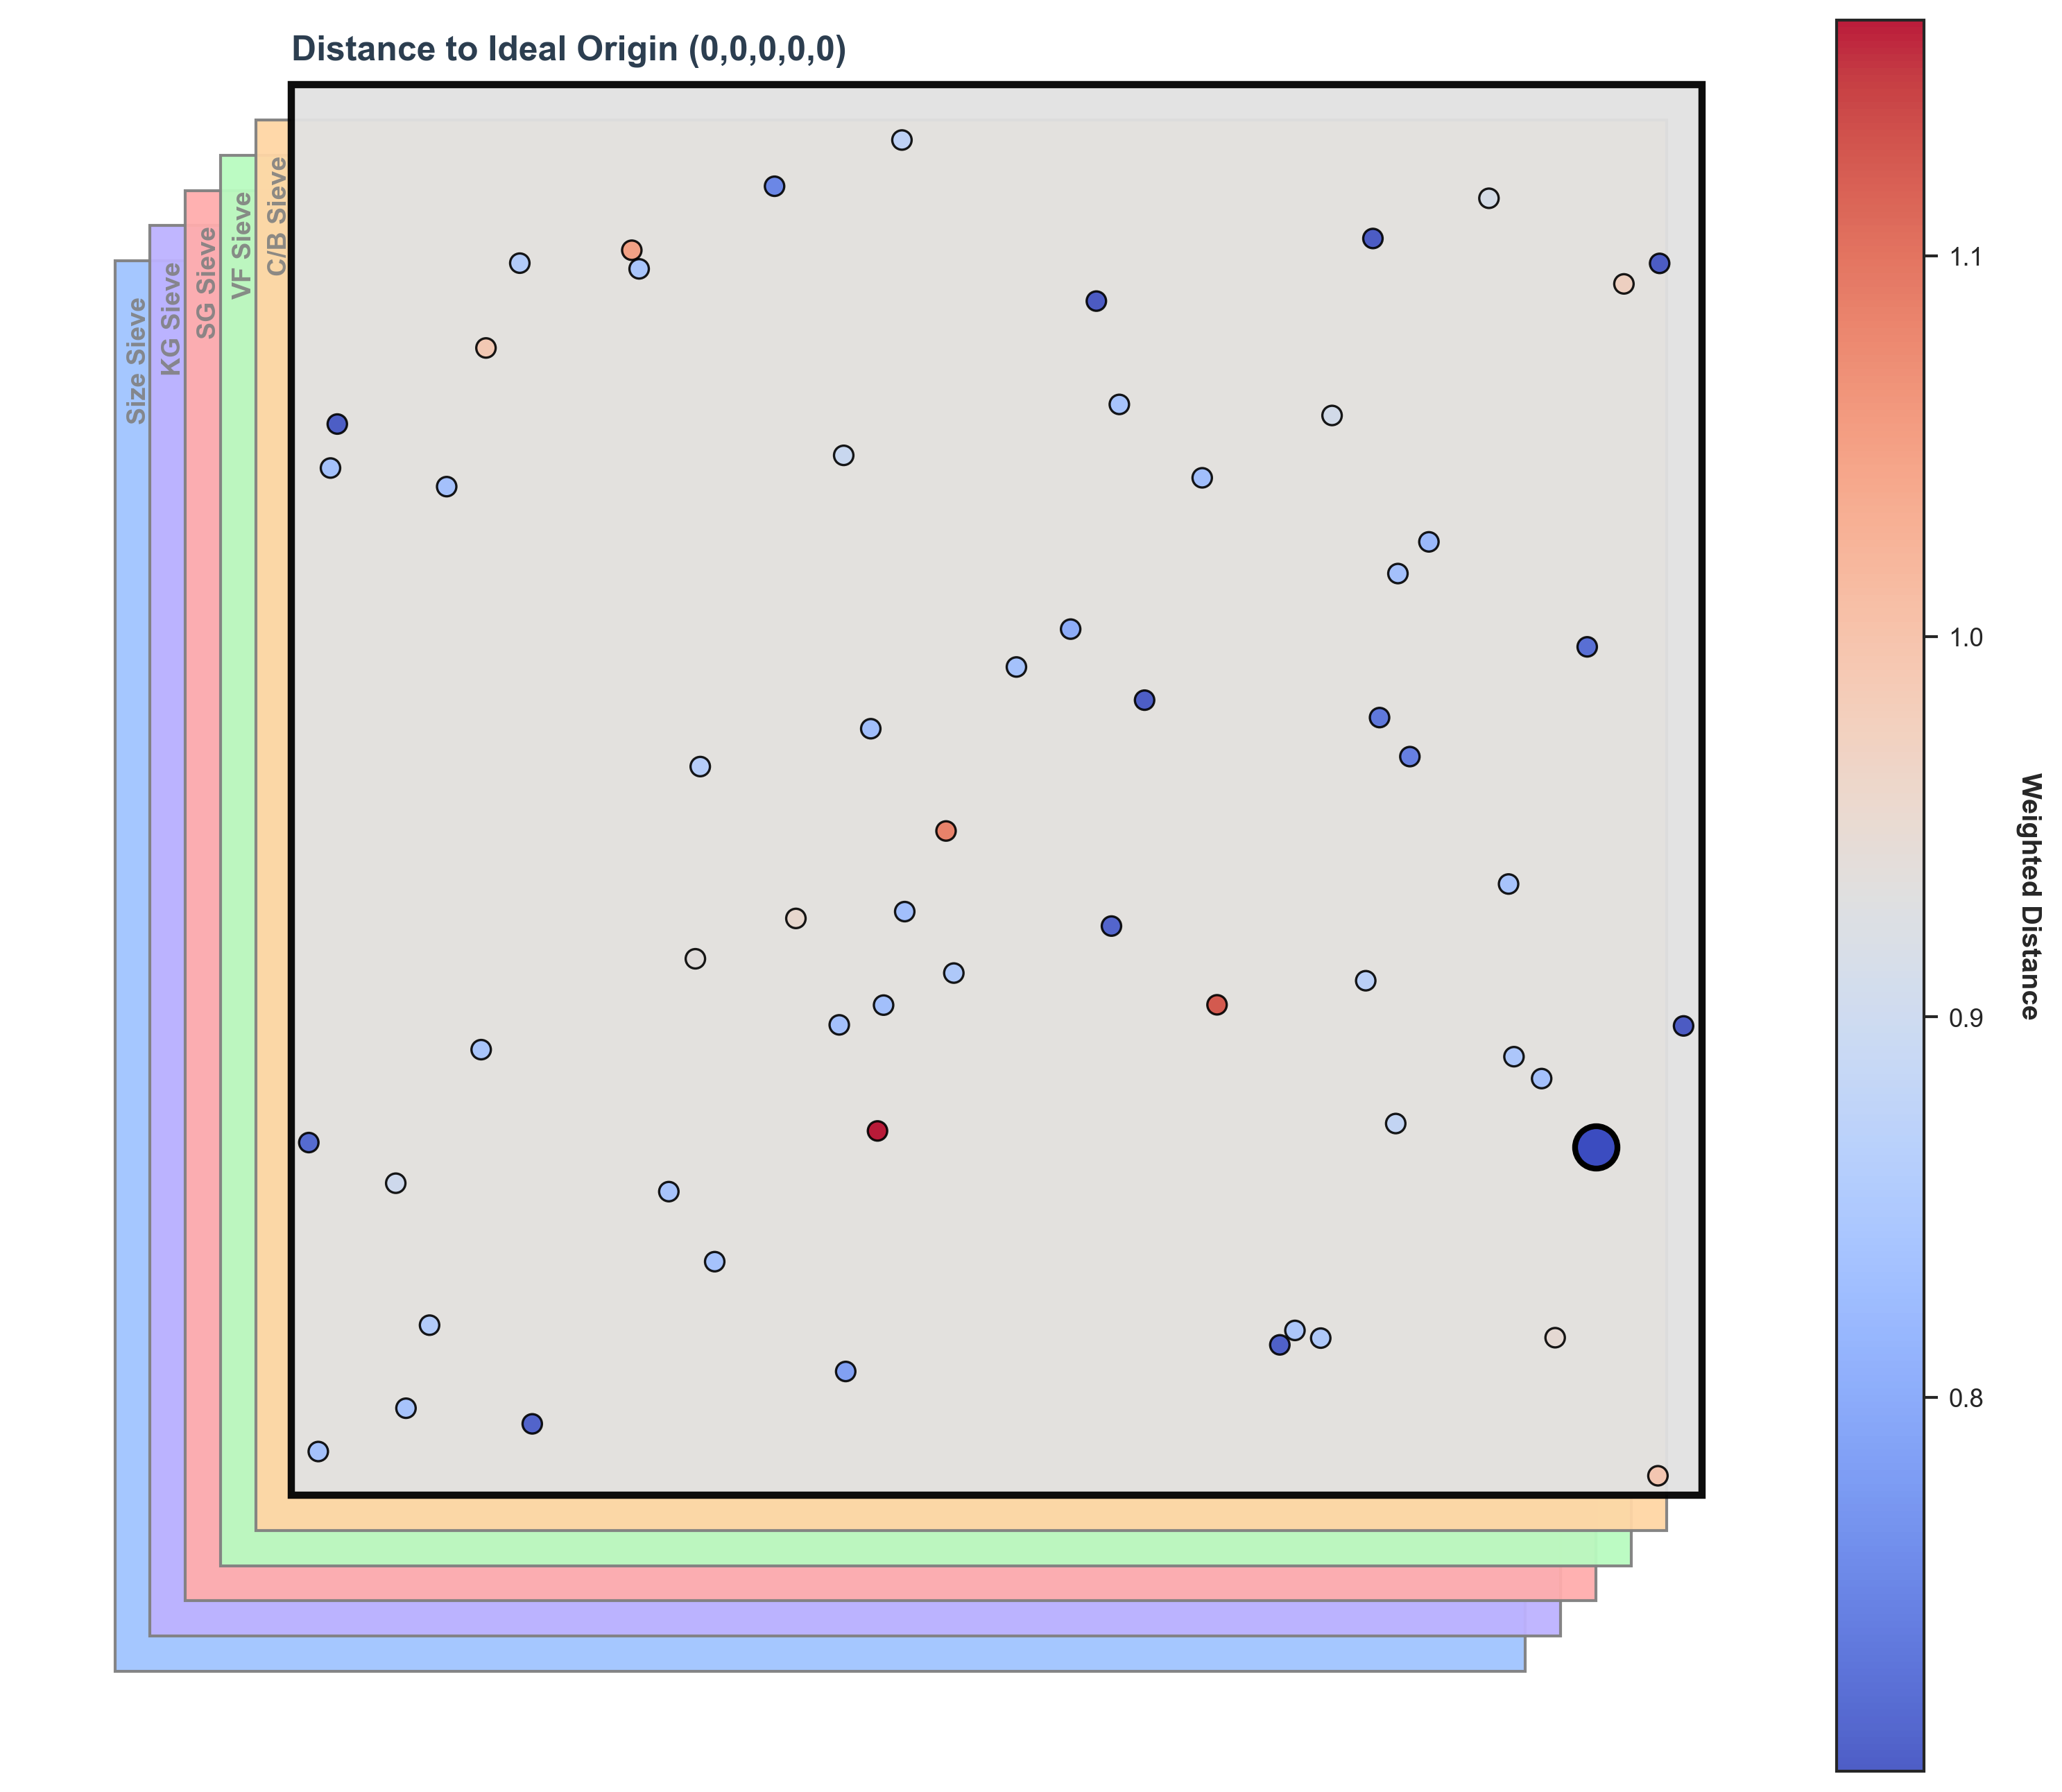
\includegraphics[width=0.7\textwidth]{content/images/sieve_step7_distance_1.png}
    \caption{Visualization of Searching for the Case 1.}
    \label{fig:distance_plot_1}
\end{figure}

The parameters and metrics values of the best candidate presented in the Table~\ref{tab:euclidean_candidate_metrics_case_1}. 


\begin{table}[htbp]
    \centering
    \small
    \caption{Performance Comparison between the Standard Baseline and the Best Shortest Distance Candidate}
    \label{tab:euclidean_candidate_metrics_case_1}
    \begin{tabular}{lrrr}
        \toprule
        \textbf{Metric} & \textbf{Standard Baseline} & \textbf{Best Candidate} & \textbf{Relative Multiplier ($X$)} \\
        \midrule
        Parameters $(h, d, k, a, w)$ & $(63, 7, 14, 12, 16)$ & $(40, 5, 19, 9, 16)$ & -- \\
        Signature Size (Bytes) & $7,872$ & $6,512$ & $0.8272\times$ \\
        Key Generation Cost & $292,862.0$ & $146,430.0$ & $0.5000\times$ \\
        Signing Cost & $2,279,391.0$ & $771,034.0$ & $0.3383\times$ \\
        Verification Cost & $2,387.0$ & $1,809.0$ & $0.7579\times$ \\
        Compression per Byte ($\rho$) & $0.303227$ & $0.277795$ & $0.9161\times$ \\
        \bottomrule
    \end{tabular}
\end{table}

\newpage

For the second case, we have the following picture:

\begin{figure}[htbp]
    \centering
    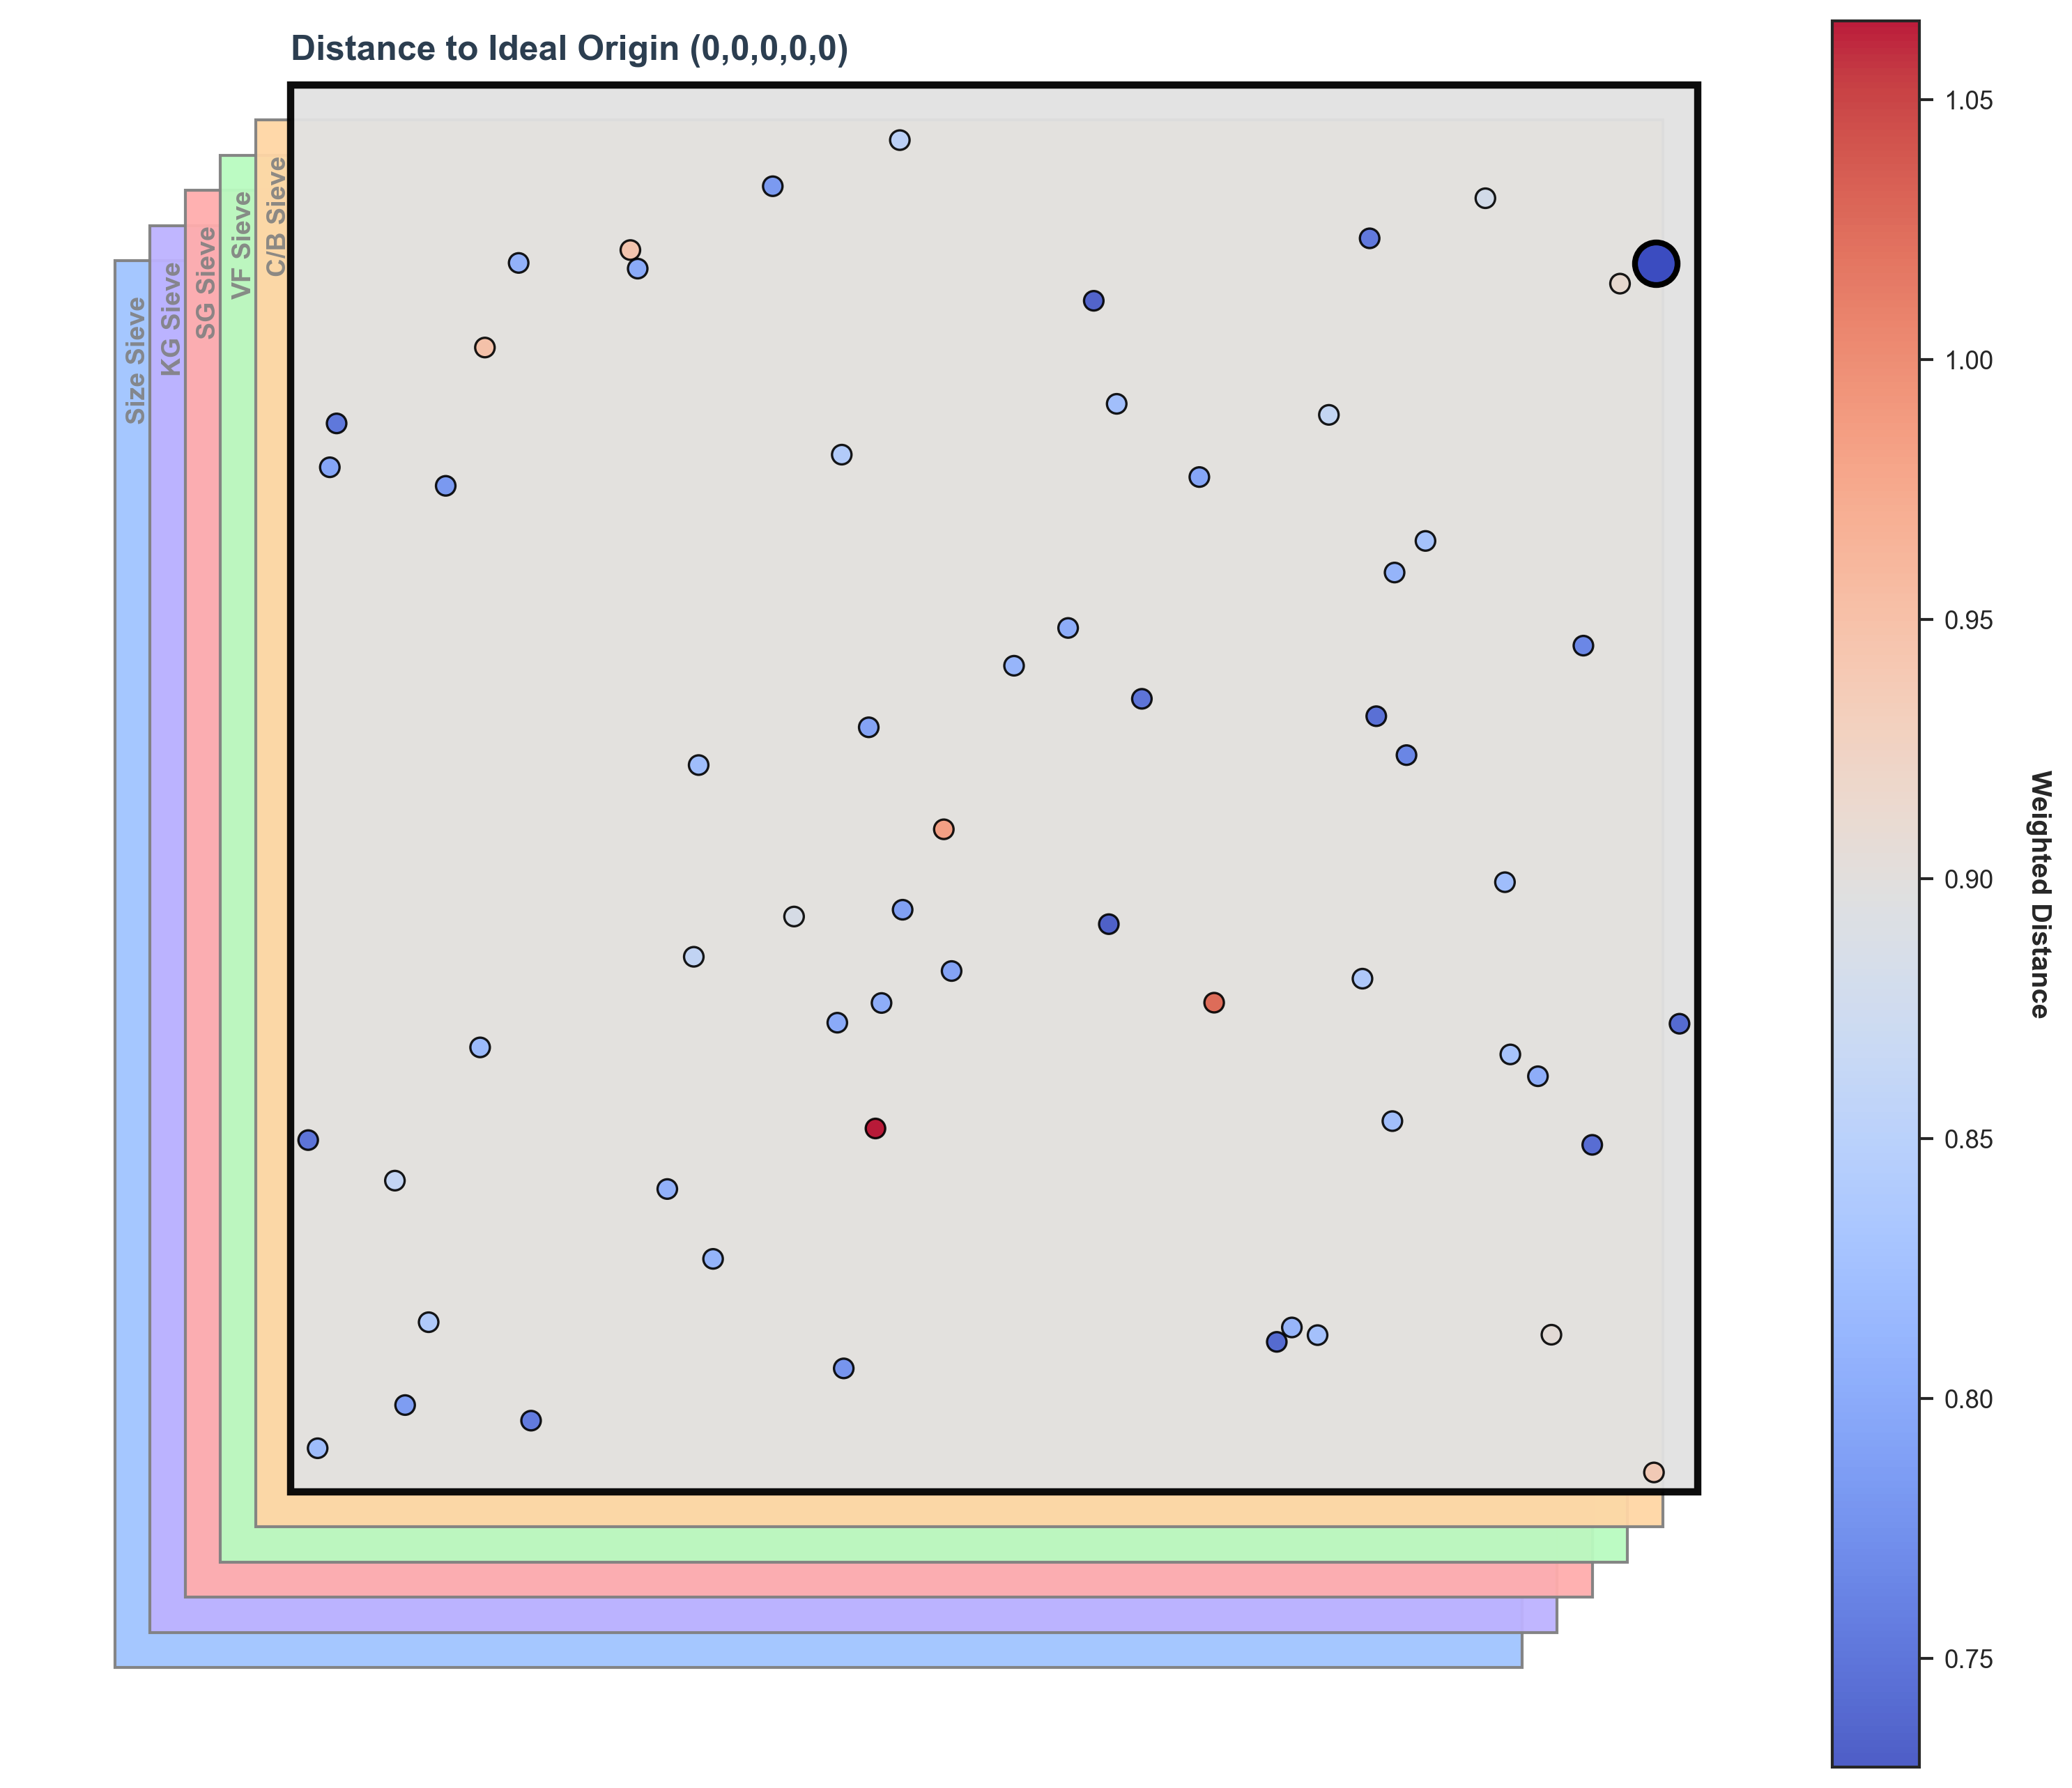
\includegraphics[width=0.75\textwidth]{content/images/sieve_step7_distance_2.png}
    \caption{Visualization of Searching for the Case 2.}
    \label{fig:distance_plot_1}
\end{figure}

And the resulting values obtained (see Table~\ref{tab:euclidean_candidate_metrics_case_2}).

\begin{table}[htbp]
    \centering
    \small
    \caption{Performance Comparison between the Standard Baseline and the Best Shortest Distance Candidate}
    \label{tab:euclidean_candidate_metrics_case_2}
    \begin{tabular}{lrrr}
        \toprule
        \textbf{Metric} & \textbf{Standard Baseline} & \textbf{Best Candidate} & \textbf{Relative Multiplier ($X$)} \\
        \midrule
        Parameters $(h, d, k, a, w)$ & $(63, 7, 14, 12, 16)$ & $(40, 5, 13, 12, 16)$ & -- \\
        Signature Size (Bytes) & $7,872$ & $6,176$ & $0.7846\times$ \\
        Key Generation Cost & $292,862.0$ & $146,430.0$ & $0.5000\times$ \\
        Signing Cost & $2,279,391.0$ & $945,124.0$ & $0.4146\times$ \\
        Verification Cost & $2,387.0$ & $1,771.0$ & $0.7419\times$ \\
        Compression per Byte ($\rho$) & $0.303227$ & $0.286755$ & $0.9457\times$ \\
        \bottomrule
    \end{tabular}
\end{table}

Comparing two cases, there is difference in the resulting metrics. While in the first case we have more balanced costs, the second case results show the prioritization for size, signing and verification. 







%% SUGGESTION: If you add \cite{} calls to the introduction (nist, delving-post,
%% conduition-blog, mike-paper), set up a bibliography here by adding a refs.bib
%% file and the following lines before \end{document}:
%%
%%     \bibliographystyle{plain}
%%     \bibliography{refs}
%%
%% Without this, every citation will render as "[?]" and latexmk will emit
%% "Citation undefined" warnings.

\end{document}